\paragraph{}Os módulos computacionais apresentados neste capítulo constituem implementações diretas das formulações matemáticas desenvolvidas no Capítulo~\ref{cap3}. Cada simulador corresponde a uma discretização específica obtida via formulação variacional de Galerkin ou, nos casos pertinentes, por diferenças finitas, e a arquitetura do software reflete o fluxo numérico subjacente: discretização espacial (MEF/MDF), montagem do sistema matricial, integração temporal e imposição das condições de contorno. Dessa forma, a estrutura da plataforma reproduz, em nível computacional, a sequência de operações matemáticas que conduz das equações governantes contínuas aos sistemas algébricos discretos efetivamente resolvidos.

\section{Visão Geral da Plataforma}
\label{sec:visao_geral}

O \textit{MinervaMesh} é uma plataforma de simulação numérica projetada para operar integralmente no navegador web, sem dependência de servidores de processamento remoto nem instalação de software por parte do usuário. A plataforma reúne implementações dos métodos numéricos apresentados no Capítulo 3 em uma interface interativa que permite a parametrização do problema, a execução da simulação e a visualização dos resultados em uma única página.

\paragraph{}A motivação central do projeto reside na eliminação das barreiras de acesso associadas às ferramentas de simulação tradicionais. Ambientes como ANSYS, COMSOL Multiphysics ou mesmo distribuições locais de Python científico exigem licenciamento, infraestrutura computacional dedicada e configuração de ambiente --- requisitos que frequentemente inviabilizam o uso autônomo em disciplinas de graduação, monitorias e estudos independentes \cite{Anjos2024}. O \textit{MinervaMesh} contorna essas limitações ao executar todo o processamento no dispositivo do próprio usuário, utilizando o navegador como ambiente de execução.

\paragraph{}A plataforma abrange três domínios da Engenharia Mecânica:
\begin{itemize}
    \item \textbf{Transferência de Calor:} condução estacionária e transiente, convecção-difusão com estabilização SUPG, transferência de calor 2D;
    \item \textbf{Mecânica dos Fluidos:} escoamento potencial, Navier-Stokes 2D via formulação Vorticidade-Corrente;
    \item \textbf{Mecânica Estrutural:} flexão de vigas (Euler-Bernoulli) e análise modal de vibração.
\end{itemize}

% Figura: Tela inicial do MinervaMesh
\begin{figure}[H]
    \centering
    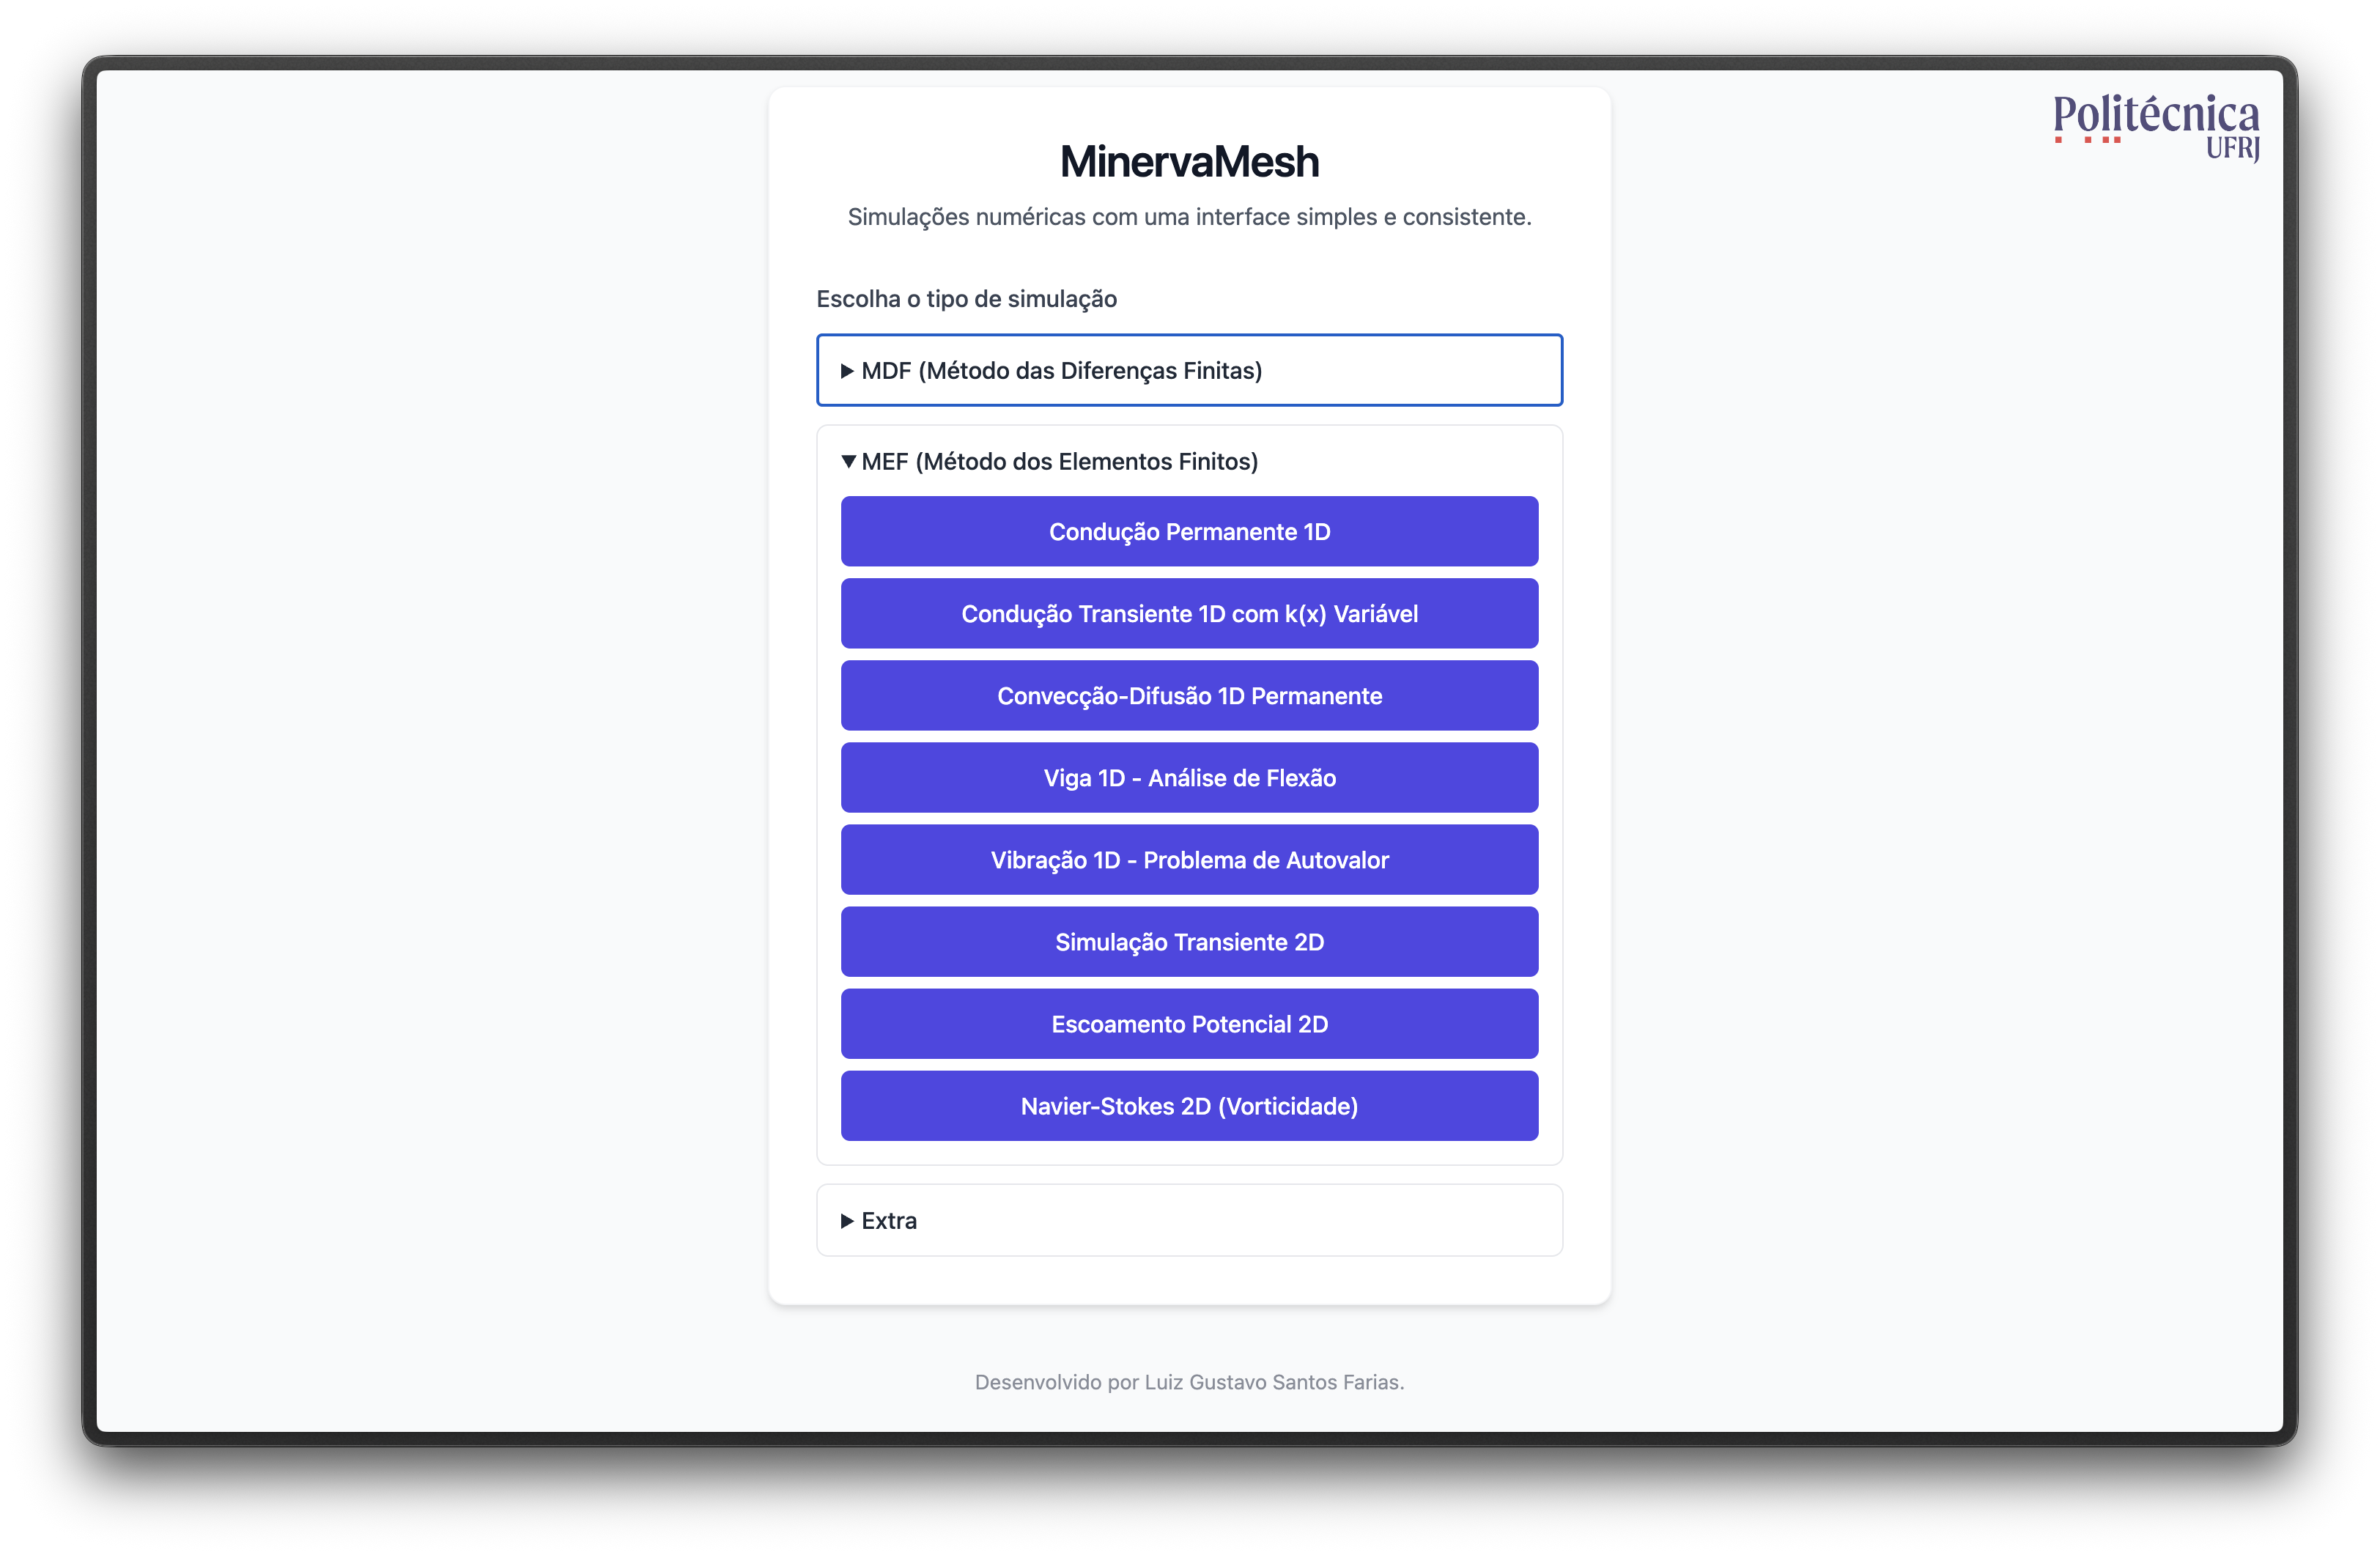
\includegraphics[width=0.9\textwidth]{figuras/prints/fig_minervamesh_home.png}
    \caption{Tela inicial do \textit{MinervaMesh} com o menu de simulações disponíveis.}
    \label{fig:minervamesh_home}
\end{figure}

\section{Justificativa Tecnológica}
\label{sec:justificativa_tecnologica}

\subsection{PyScript e WebAssembly}
\label{sec:pyscript}

A escolha do PyScript como runtime da plataforma fundamenta-se em três critérios: portabilidade, familiaridade da linguagem e manutenibilidade.

\paragraph{}O PyScript é um \textit{framework} de código aberto que permite a execução de programas Python diretamente no navegador, apoiando-se no Pyodide --- uma compilação do interpretador CPython para WebAssembly (Wasm) \cite{PyScript2023}. O WebAssembly é um formato binário padronizado pelo W3C que executa código de baixo nível em velocidade próxima à nativa, dentro da \textit{sandbox} de segurança do navegador. A cadeia de execução é:

\begin{enumerate}
    \item O navegador carrega a página HTML contendo a tag \texttt{<script type="py">}.
    \item O \textit{runtime} do PyScript inicializa o Pyodide, que instancia uma máquina virtual CPython compilada para WebAssembly.
    \item As dependências declaradas em \texttt{config.toml} (NumPy, SciPy, Matplotlib) são carregadas como pacotes pré-compilados para Wasm.
    \item O código Python da simulação é interpretado pelo Pyodide, com acesso direto ao DOM do navegador para leitura de parâmetros e renderização de resultados.
\end{enumerate}

\paragraph{}A escolha de Python como linguagem de implementação é estratégica para o contexto educacional: a linguagem apresenta sintaxe próxima à notação matemática e dispõe de um ecossistema científico consolidado --- NumPy para álgebra linear, SciPy para solvers esparsos, Matplotlib para visualização \cite{Harris2020}. Ao manter a implementação em Python puro, o \textit{MinervaMesh} permite que alunos inspecionem, compreendam e modifiquem o código das simulações --- funcionalidade explicitamente disponível através do botão ``Ver Código'' presente em cada simulação.

\subsection{Computação \textit{Client-Side}}
\label{sec:client_side}

A arquitetura \textit{client-side} implica que todo o processamento numérico ocorre no dispositivo do usuário. Esta decisão tem impactos diretos em quatro dimensões:

\begin{enumerate}
    \item \textbf{Custo de infraestrutura:} o \textit{MinervaMesh} é um site estático. Pode ser hospedado gratuitamente em plataformas como GitHub Pages ou Netlify, sem necessidade de servidor \textit{backend}, banco de dados ou infraestrutura de \textit{cloud computing}. O custo operacional é efetivamente zero.
    \item \textbf{Escalabilidade:} não existe gargalo de servidor central. Cada usuário utiliza o poder computacional de sua própria máquina, eliminando filas de processamento e limites de usuários simultâneos.
    \item \textbf{Privacidade:} nenhum dado de simulação transita pela rede. Parâmetros, malhas e resultados permanecem integralmente no dispositivo do usuário.
    \item \textbf{Disponibilidade:} após o carregamento inicial dos \textit{assets}, a plataforma pode operar sem conexão com a internet, viabilizando o uso em ambientes com conectividade limitada.
\end{enumerate}

\subsection{Comparação com Alternativas}
\label{sec:comparacao_alternativas}

A Tabela \ref{tab:comparacao_plataformas} posiciona o \textit{MinervaMesh} frente às alternativas mais comuns no contexto de ensino de simulação numérica.

\begin{table}[H]
\centering
\caption{Comparação entre plataformas de simulação numérica para ensino.}
\label{tab:comparacao_plataformas}
\begin{tabular}{lccccc}
\hline
\textbf{Critério} & \textbf{MinervaMesh} & \textbf{MATLAB} & \textbf{Jupyter} & \textbf{COMSOL} \\
\hline
Custo de licença           & Gratuito & Pago       & Gratuito   & Pago \\
Instalação necessária      & Não      & Sim        & Sim        & Sim \\
Execução no navegador      & Sim      & Não        & Parcial    & Não \\
Código-fonte acessível     & Sim      & Parcial    & Sim        & Não \\
Infraestrutura de servidor & Não      & Não        & Sim        & Sim \\
\hline
\end{tabular}
\end{table}

A principal limitação da abordagem \textit{client-side} reside na capacidade computacional: problemas com malhas muito refinadas (dezenas de milhares de nós) podem apresentar tempo de execução elevado, uma vez que o desempenho do WebAssembly, embora próximo ao nativo, ainda é inferior ao de implementações compiladas em C/Fortran. Para os casos de interesse deste trabalho, envolvendo malhas de centenas a poucos milhares de nós, essa limitação não se mostrou restritiva.

\section{Arquitetura de Software}
\label{sec:arquitetura_software}

\subsection{Organização de Diretórios}
\label{sec:organizacao_diretorios}

O repositório do \textit{MinervaMesh} segue uma estrutura modular, onde cada simulação é autocontida em seu próprio diretório. A organização geral é apresentada a seguir:

\begin{lstlisting}[style=dirstyle,numbers=none]
minervamesh/
|-- index.html                    # Menu principal
|-- assets/                       # Logos e imagens globais
|-- simulations/
|   |-- mef/                     # Elementos Finitos
|   |   |-- <nome-do-modulo>/
|   |   |   |-- index.html       # Interface do usuario
|   |   |   |-- simulation.py    # Logica numerica
|   |   |   +-- config.toml      # Dependencias Python
|   |   |-- ...                  # (8 modulos MEF)
|   |   +-- escoamento-fluido-2d/
|   |       |-- common.py        # Matrizes MEF 2D
|   |       +-- geometry.py      # Geometrias de obstaculo
|   |-- mdf/                     # Diferencas Finitas
|   +-- extra/                   # Ferramentas auxiliares
\end{lstlisting}

Cada módulo de simulação segue um padrão uniforme de três arquivos:
\begin{itemize}
    \item \texttt{index.html}: interface do usuário, contendo o formulário de parâmetros, o contêiner de resultados e a carga do PyScript;
    \item \texttt{simulation.py}: implementação da lógica numérica em Python, incluindo montagem de matrizes, solução do sistema e geração de gráficos;
    \item \texttt{config.toml}: declaração das dependências Python necessárias (por exemplo, \texttt{numpy}, \texttt{scipy}, \texttt{matplotlib}).
\end{itemize}

\subsection{Fluxo de Execução de uma Simulação}
\label{sec:fluxo_execucao}

O ciclo de vida de uma simulação no \textit{MinervaMesh} pode ser descrito em cinco etapas:

\begin{enumerate}
    \item \textbf{Carregamento:} o navegador requisita o \texttt{index.html} de um servidor HTTP simples. A tag \texttt{<script type="py">} instrui o PyScript a inicializar o Pyodide e carregar as dependências declaradas em \texttt{config.toml}.
    \item \textbf{Parametrização:} o usuário configura os parâmetros físicos e numéricos através de campos de entrada na interface.
    \item \textbf{Execução:} ao clicar em ``Rodar'', o código Python é executado pelo Pyodide. As matrizes do MEF são montadas, o sistema linear é resolvido e os gráficos são gerados --- tudo no navegador.
    \item \textbf{Visualização:} os gráficos resultantes são convertidos para formato de imagem codificado em Base64 e inseridos dinamicamente no DOM da página.
    \item \textbf{Inspeção:} o botão ``Ver Código'' exibe o código-fonte Python da simulação com \textit{syntax highlighting}, permitindo ao aluno estudar a implementação.
\end{enumerate}

\begin{figure}[H]
    \centering
    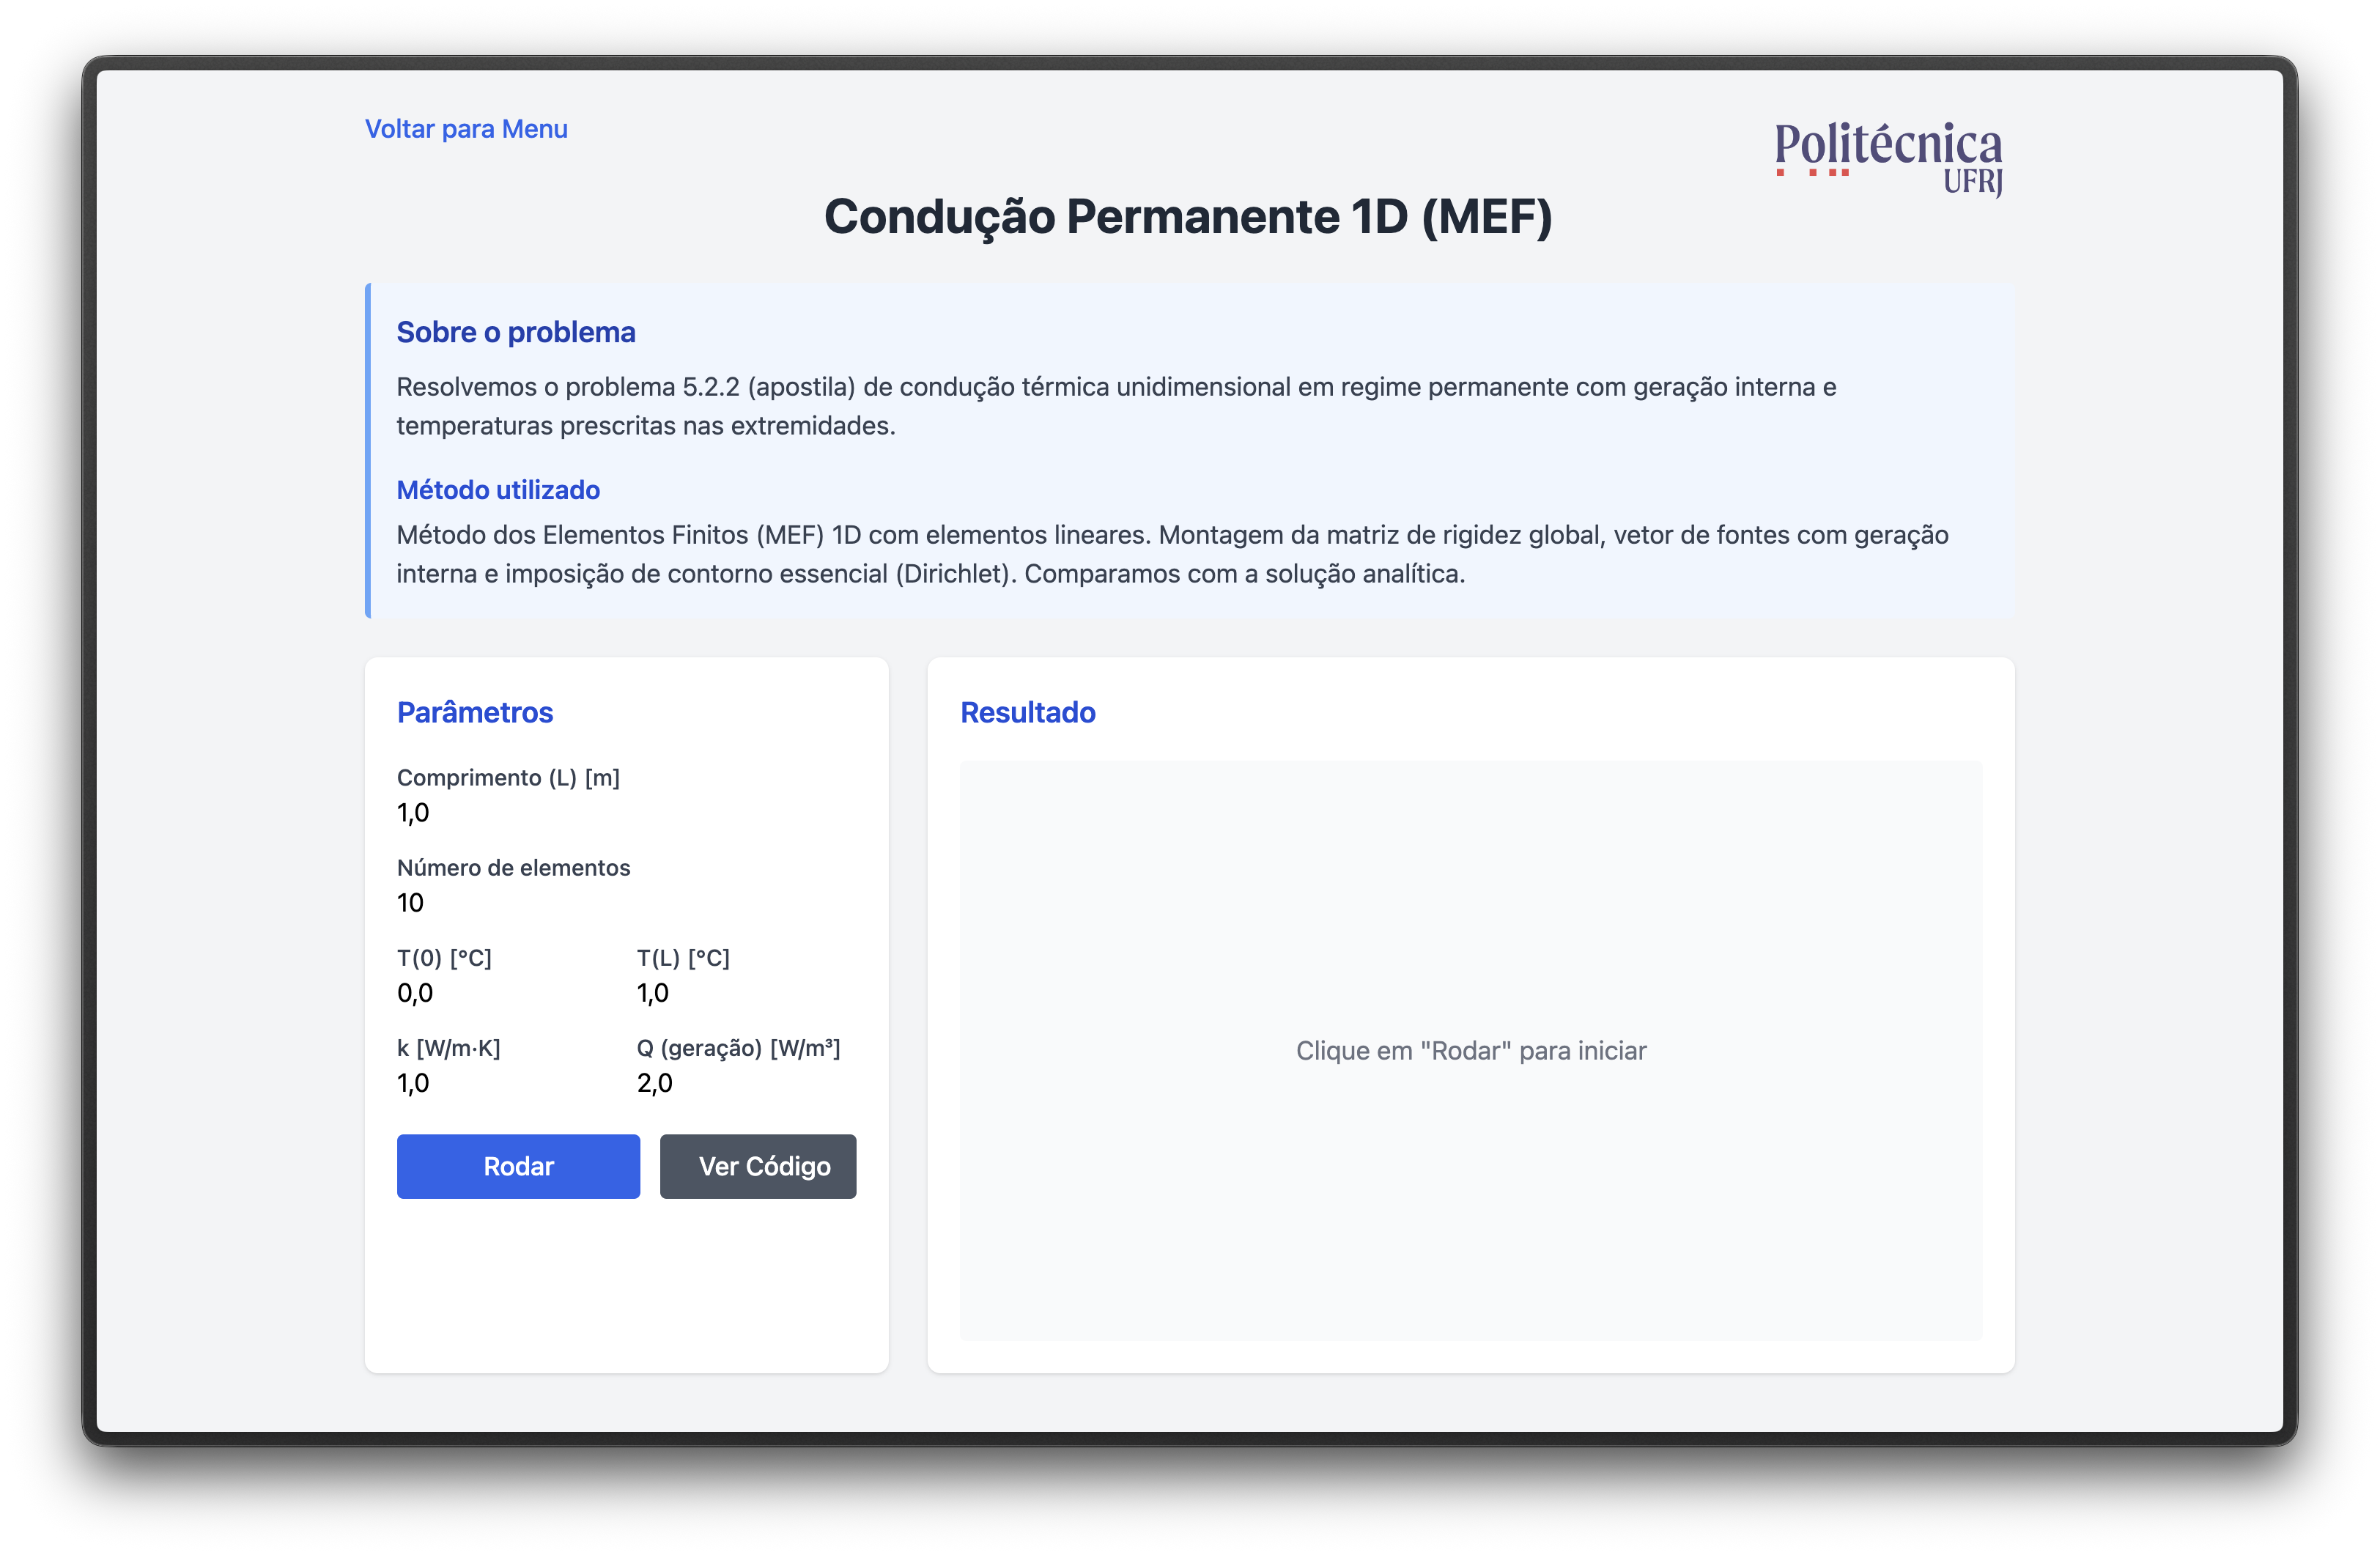
\includegraphics[width=0.9\textwidth]{figuras/prints/fig_interface_parametros.png}
    \caption{Interface de parametrização de uma simulação (Condução Permanente 1D) antes da execução.}
    \label{fig:interface_parametros}
\end{figure}

\section{Módulos de Simulação MEF}
\label{sec:modulos_mef}

Esta seção descreve cada módulo de simulação implementado no \textit{MinervaMesh}, detalhando o problema físico resolvido, as decisões de implementação e os resultados obtidos. Os trechos de código apresentados referem-se às funções centrais de cada simulação; as listagens completas encontram-se nos Apêndices.

\paragraph{}Todos os módulos implementam diretamente as formulações variacionais e discretizações desenvolvidas no Capítulo~\ref{cap3}. As matrizes elementares de rigidez, massa e carga são construídas a partir das expressões derivadas nas Seções~\ref{sec:matrizes_elementares} e~\ref{sec:supg}, e cada trecho de código apresentado nesta seção referencia explicitamente a equação teórica correspondente, mantendo correspondência direta entre operadores matemáticos e operadores numéricos.

\subsection{Condução Permanente 1D}
\label{sec:caso_conducao_1d}

O primeiro módulo resolve o problema de condução térmica unidimensional em regime permanente com geração interna de calor. A equação governante é a forma 1D da equação de Poisson (Eq.~\ref{eq:conducao_geral} com $\partial T / \partial t = 0$):

\begin{equation}
-k \frac{d^2 T}{dx^2} = Q, \quad T(0) = T_0, \quad T(L) = T_L
\label{eq:conducao_1d_caso}
\end{equation}

A discretização por elementos finitos lineares resulta na matriz de rigidez e no vetor de carga elementares (Seção \ref{sec:matrizes_elementares}), implementados como:

\begin{lstlisting}
# Elemento linear 1D: ke e be
ke = (k / h) * np.array([[1.0, -1.0], [-1.0, 1.0]])
be = (Q * h / 2.0) * np.array([1.0, 1.0])
\end{lstlisting}

A montagem percorre os $N_{el}$ elementos, acumulando as contribuições nas posições globais. Após a imposição das condições de Dirichlet (zerando linhas e colunas correspondentes), o sistema $\mathbf{K}\mathbf{T} = \mathbf{b}$ é resolvido por \texttt{numpy.linalg.solve}. A Figura \ref{fig:conducao1d_resultado} mostra a comparação entre a solução MEF e a solução analítica.

\begin{figure}[H]
    \centering
    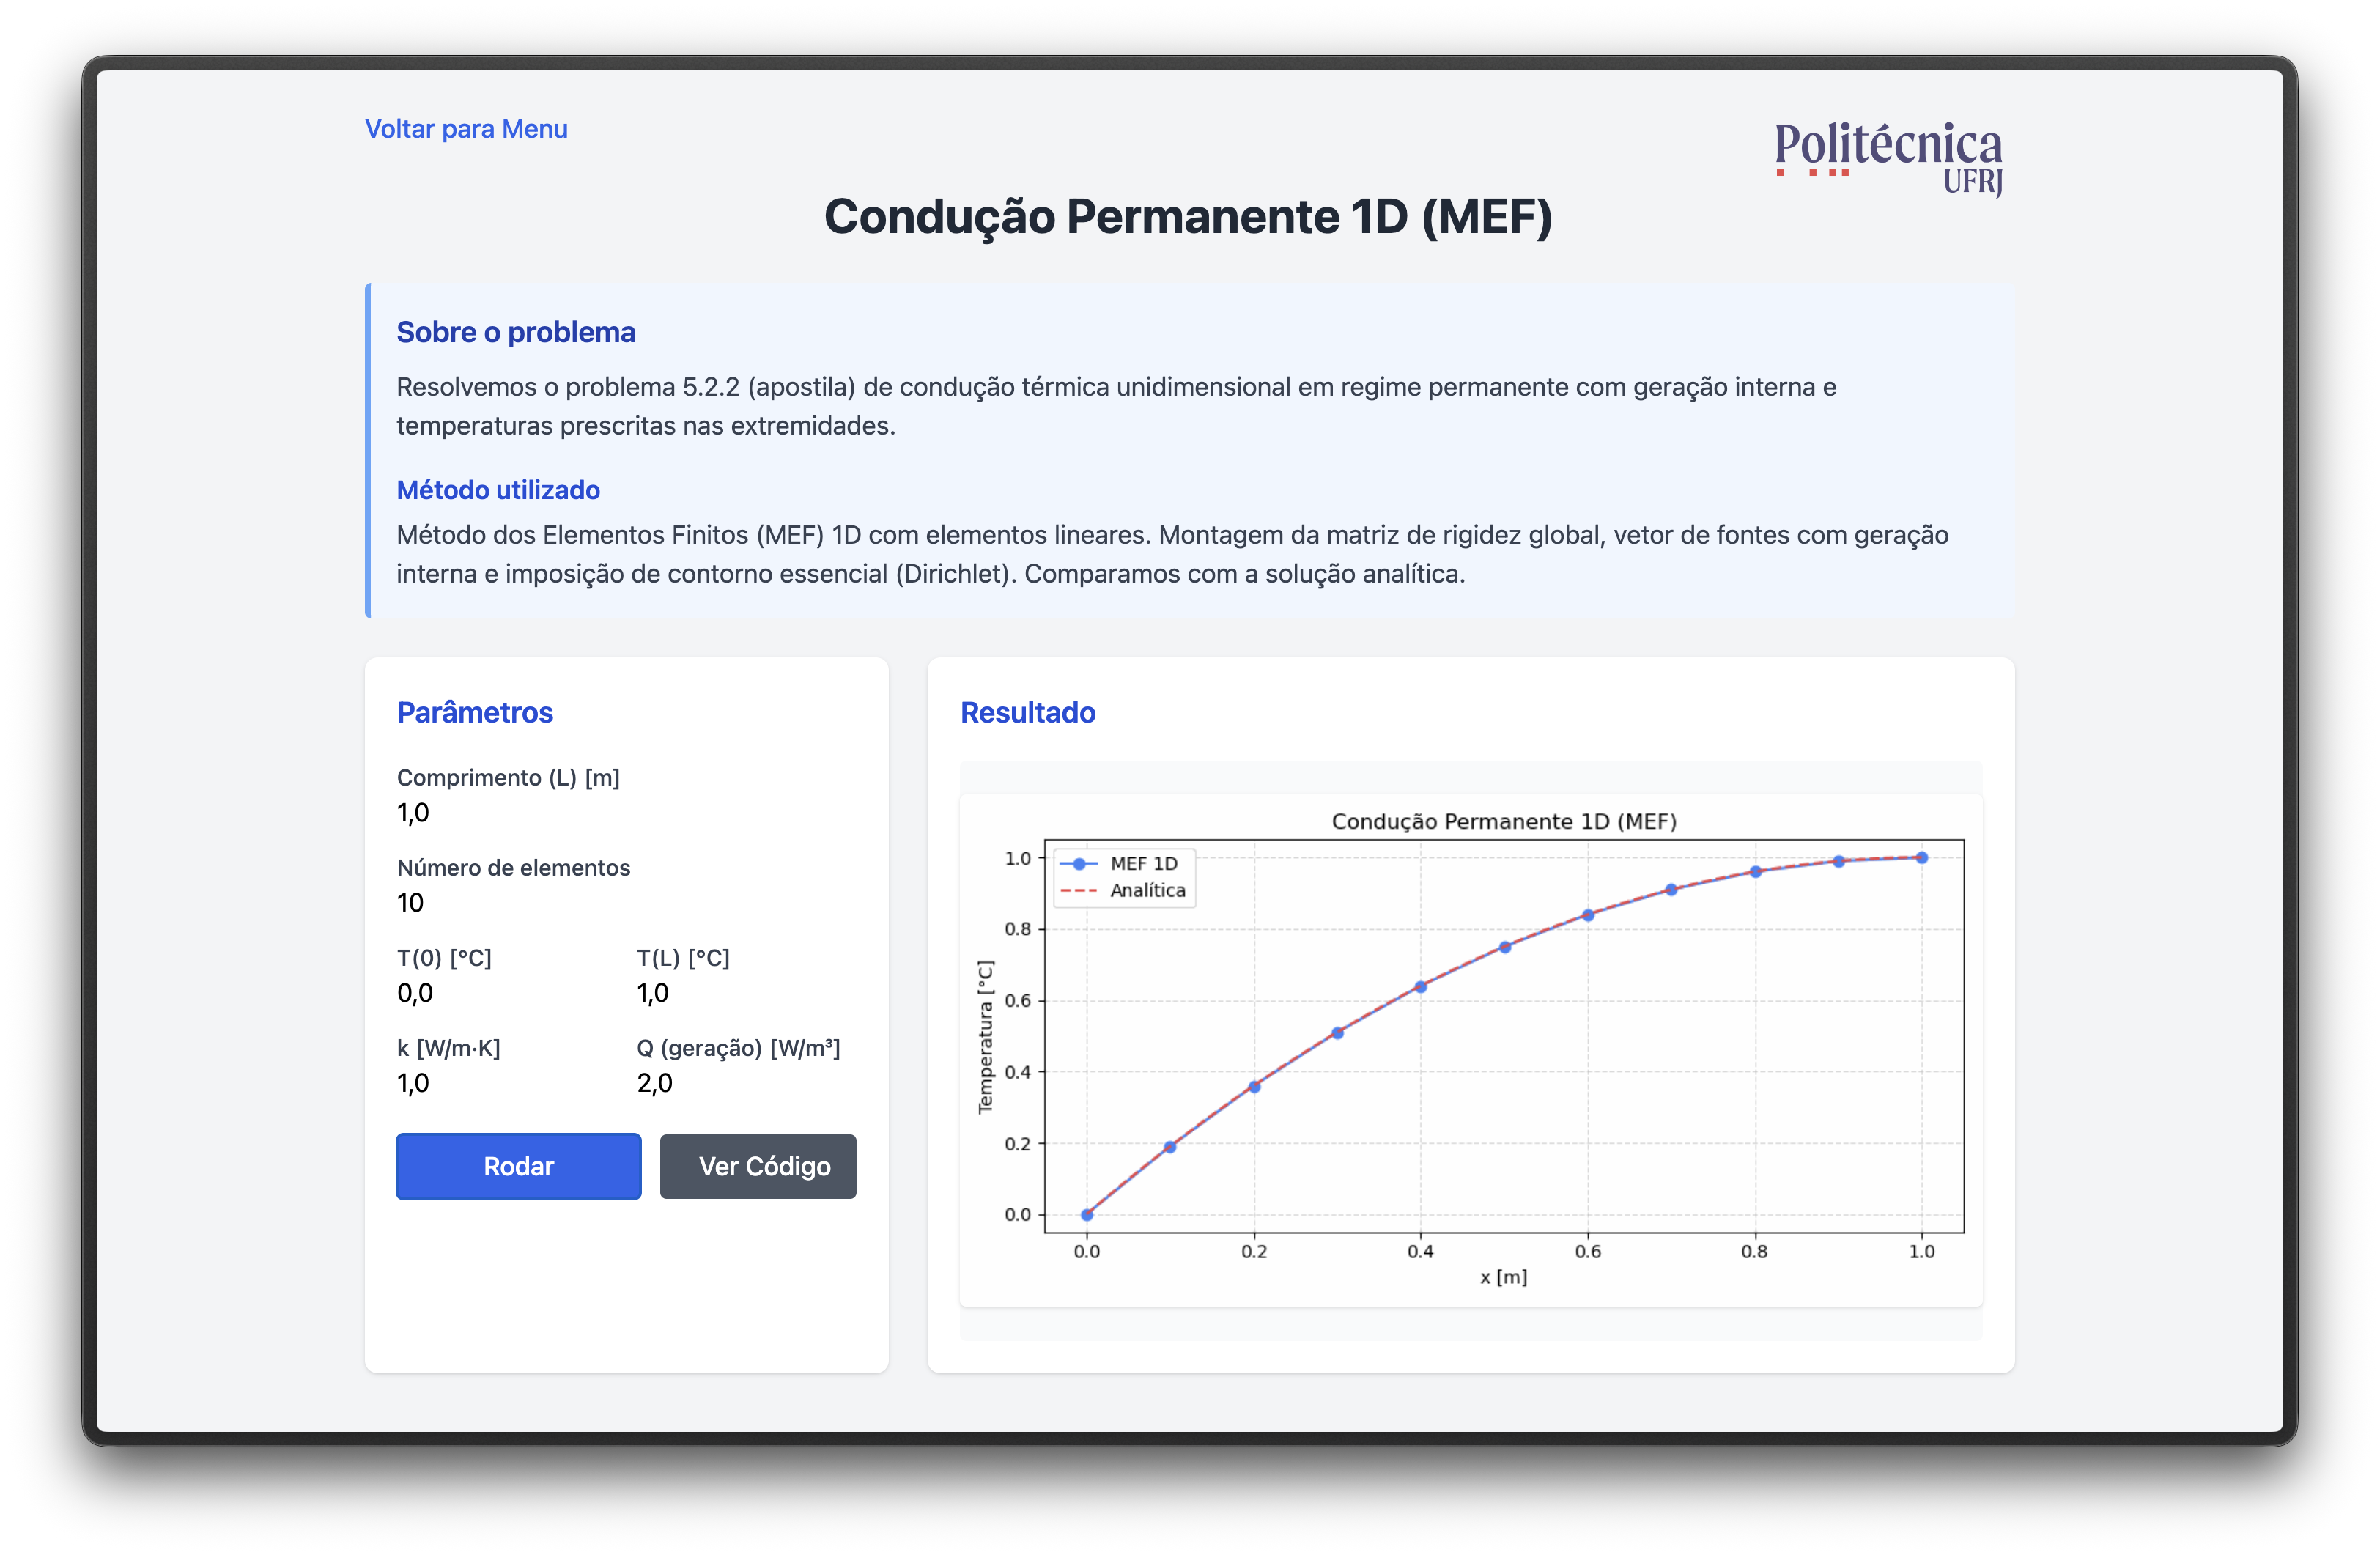
\includegraphics[width=0.85\textwidth]{figuras/prints/fig_conducao1d_resultado.png}
    \caption{Condução permanente 1D: solução MEF ($N_{el}=10$) comparada à solução analítica.}
    \label{fig:conducao1d_resultado}
\end{figure}

\subsection{Condução Transiente 1D com $k(x)$ Variável}
\label{sec:caso_calor_transiente}

Este módulo estende o problema anterior para o regime transiente, incorporando a matriz de massa e a integração temporal conforme o sistema semidiscreto estabelecido na Seção~\ref{sec:integracao_temporal}. A equação governante é:

\begin{equation}
\rho c_p \frac{\partial T}{\partial t} = \frac{\partial}{\partial x}\left( k(x) \frac{\partial T}{\partial x} \right)
\label{eq:transiente_1d_caso}
\end{equation}
com condutividade térmica variável $k(x)$, definida como $k_1 = 5{,}0$ para $x < L/2$ e $k_2 = 1{,}0$ para $x \geq L/2$.

As matrizes elementares são calculadas por:

\begin{lstlisting}
# Matrizes de elemento 1D transiente
ke = (k_avg / h) * np.array([[1, -1], [-1, 1]])
me = (rho_cp * h / 6) * np.array([[2, 1], [1, 2]])
\end{lstlisting}

A integração temporal utiliza o método $\theta$ generalizado (Eq.~\ref{eq:theta_method}), seguindo rigorosamente o esquema de avanço temporal derivado na Seção~\ref{sec:integracao_temporal}, e permitindo ao usuário selecionar entre Euler explícito, Crank-Nicolson e Euler implícito. A Figura \ref{fig:calor_transiente1d} ilustra a evolução temporal do campo de temperatura.

\begin{figure}[H]
    \centering
    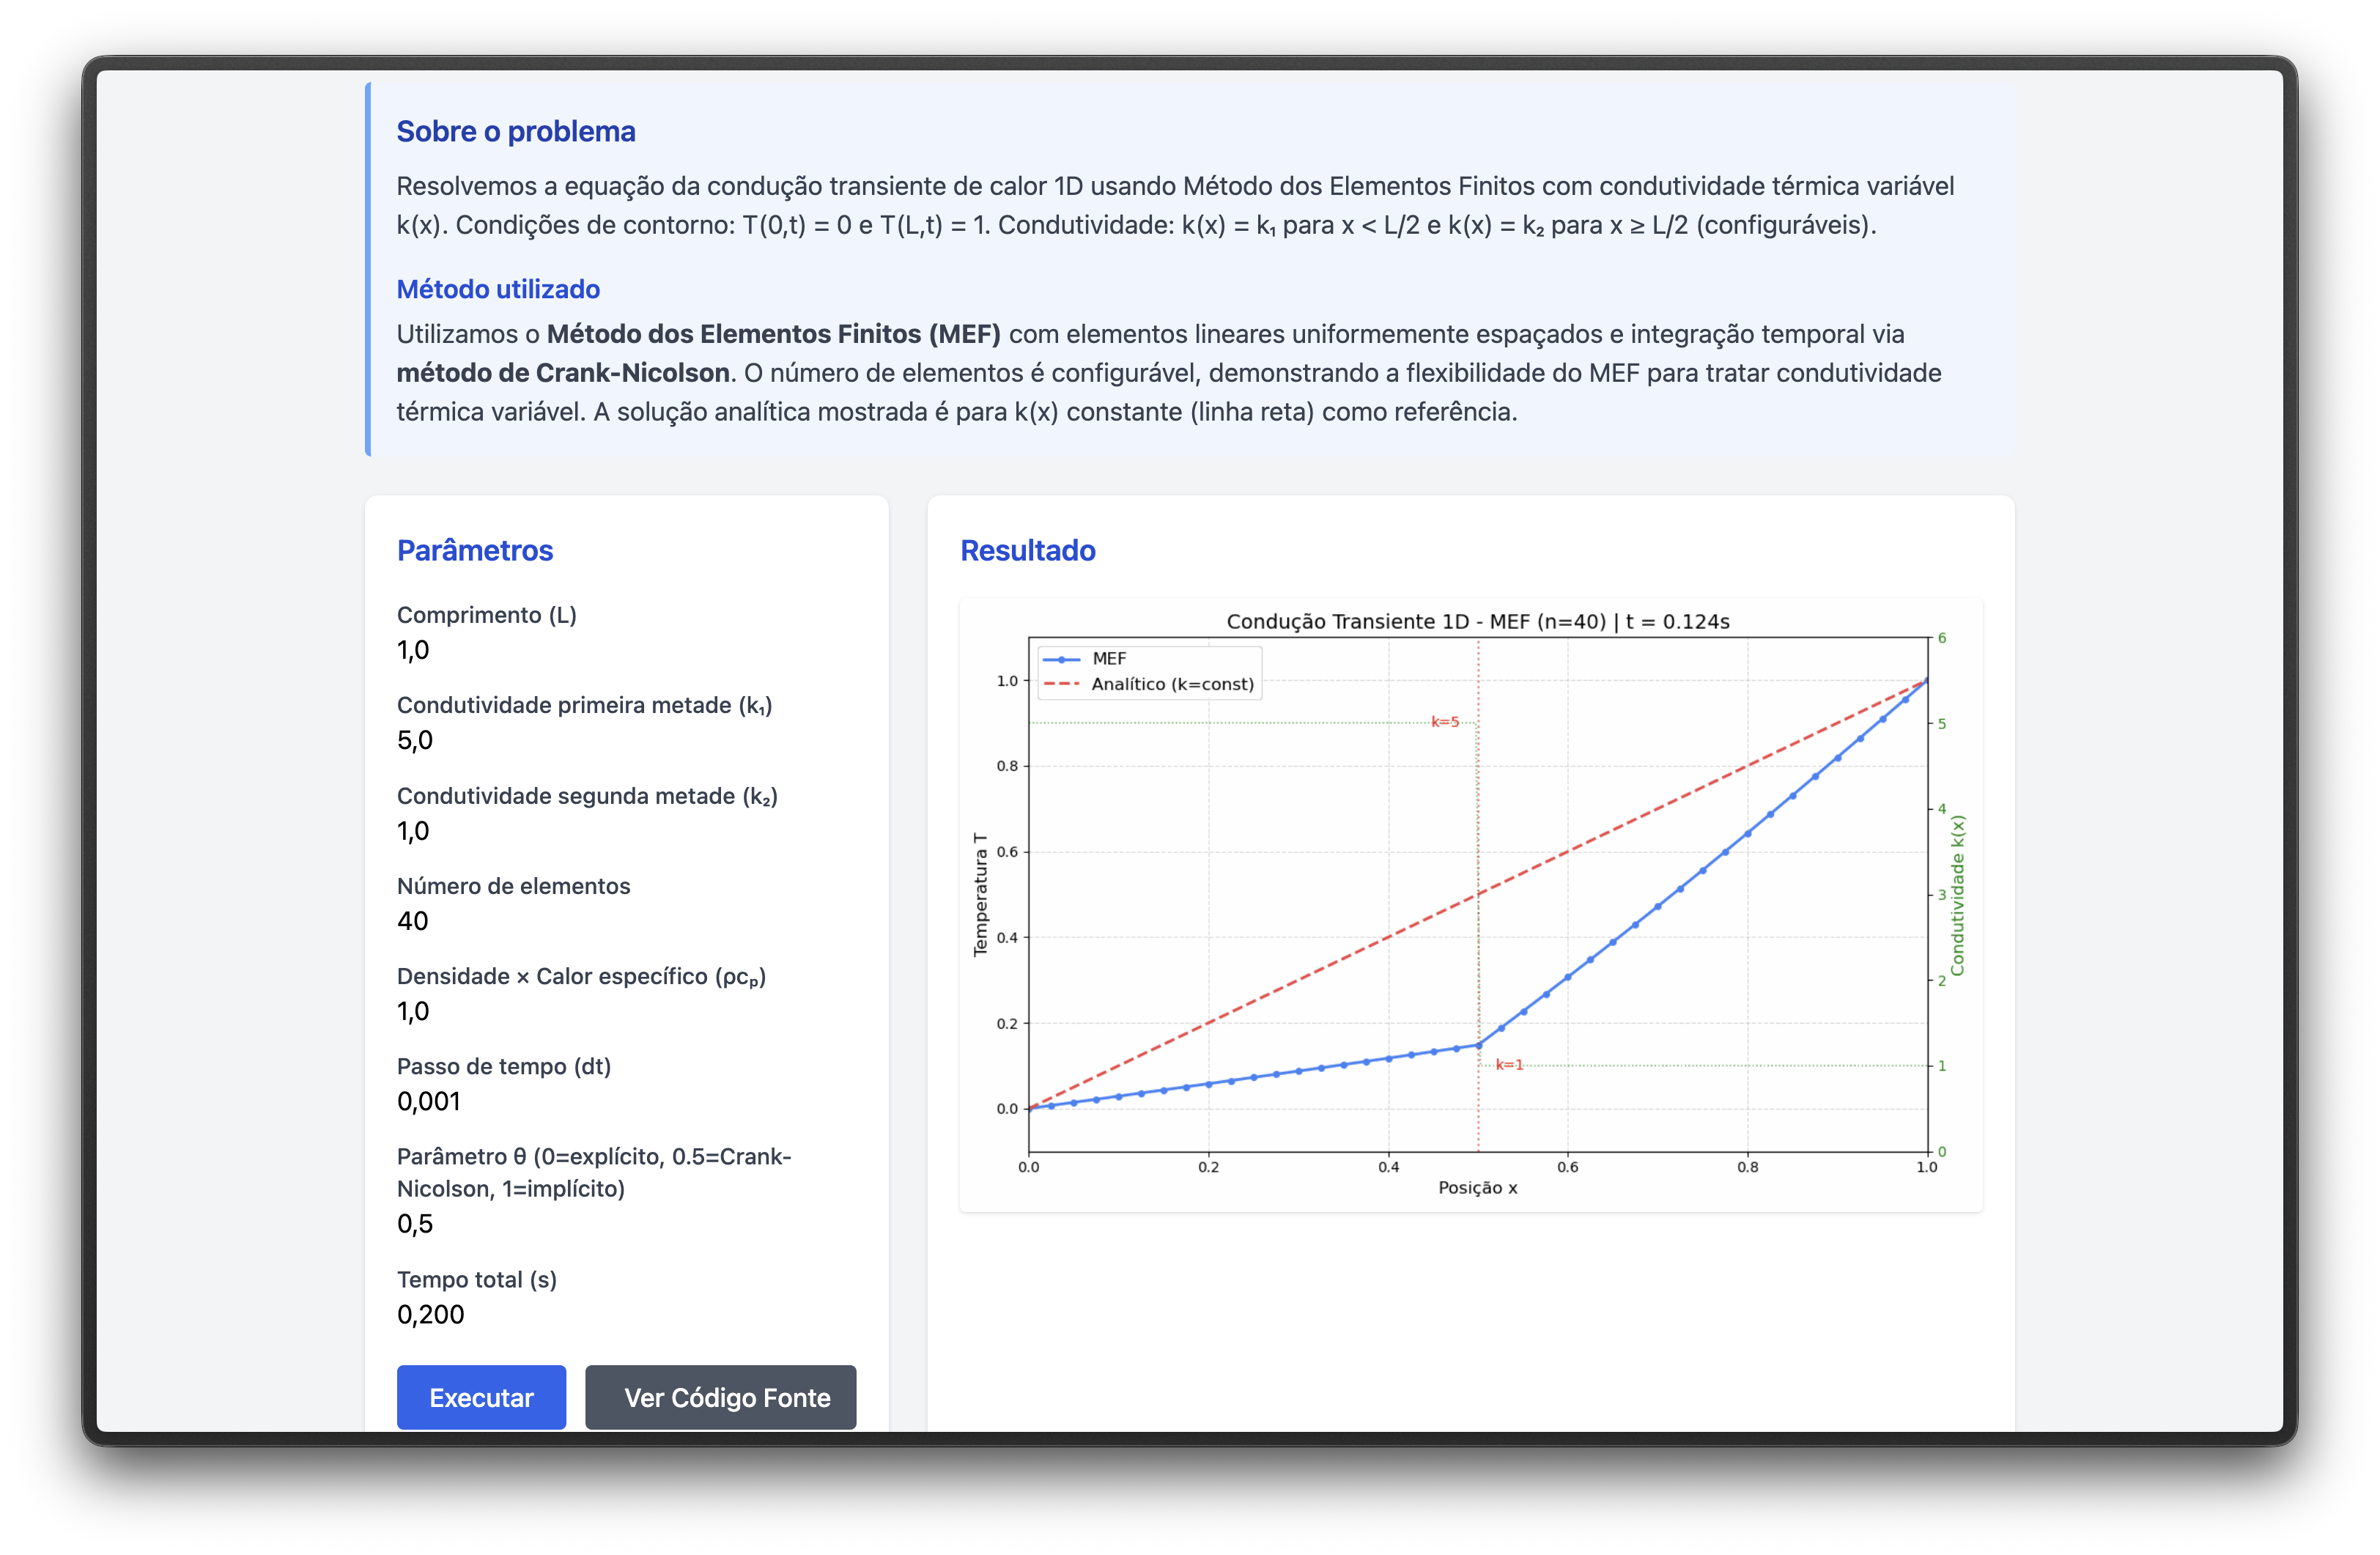
\includegraphics[width=0.85\textwidth]{figuras/prints/fig_calor_transiente1d_evolucao.png}
    \caption{Evolução temporal do campo de temperatura com condutividade variável $k(x)$.}
    \label{fig:calor_transiente1d}
\end{figure}

\subsection{Convecção-Difusão 1D com Estabilização SUPG}
\label{sec:caso_convdif}

O módulo de convecção-difusão 1D resolve a equação de advecção-difusão estacionária, aplicando a técnica de estabilização SUPG conforme a formulação desenvolvida na Seção~\ref{sec:supg}:

\begin{equation}
-k \frac{d^2 T}{dx^2} + \rho c_p \, u \frac{dT}{dx} = Q
\label{eq:convdif_1d_caso}
\end{equation}

A discretização MEF gera três matrizes elementares: difusão, convecção e estabilização SUPG (Seção~\ref{sec:supg}). O parâmetro $\tau_{\text{SUPG}}$ é calculado segundo a expressão analítica da Eq.~\ref{eq:tau_supg}, implementado como:

\begin{lstlisting}
# Numero de Peclet local e tau SUPG
Pe_local = (rho_cp * u * h) / (2 * k)
tau = h / (2*abs(u)) * (1/np.tanh(abs(Pe_local))
                        - 1/abs(Pe_local))
\end{lstlisting}

A Figura \ref{fig:convdif_supg} demonstra o efeito da estabilização SUPG em um problema com número de Péclet elevado. Sem estabilização, a formulação de Galerkin padrão produz oscilações espúrias; com SUPG, a solução numérica converge suavemente para a solução analítica.

\begin{figure}[H]
    \centering
    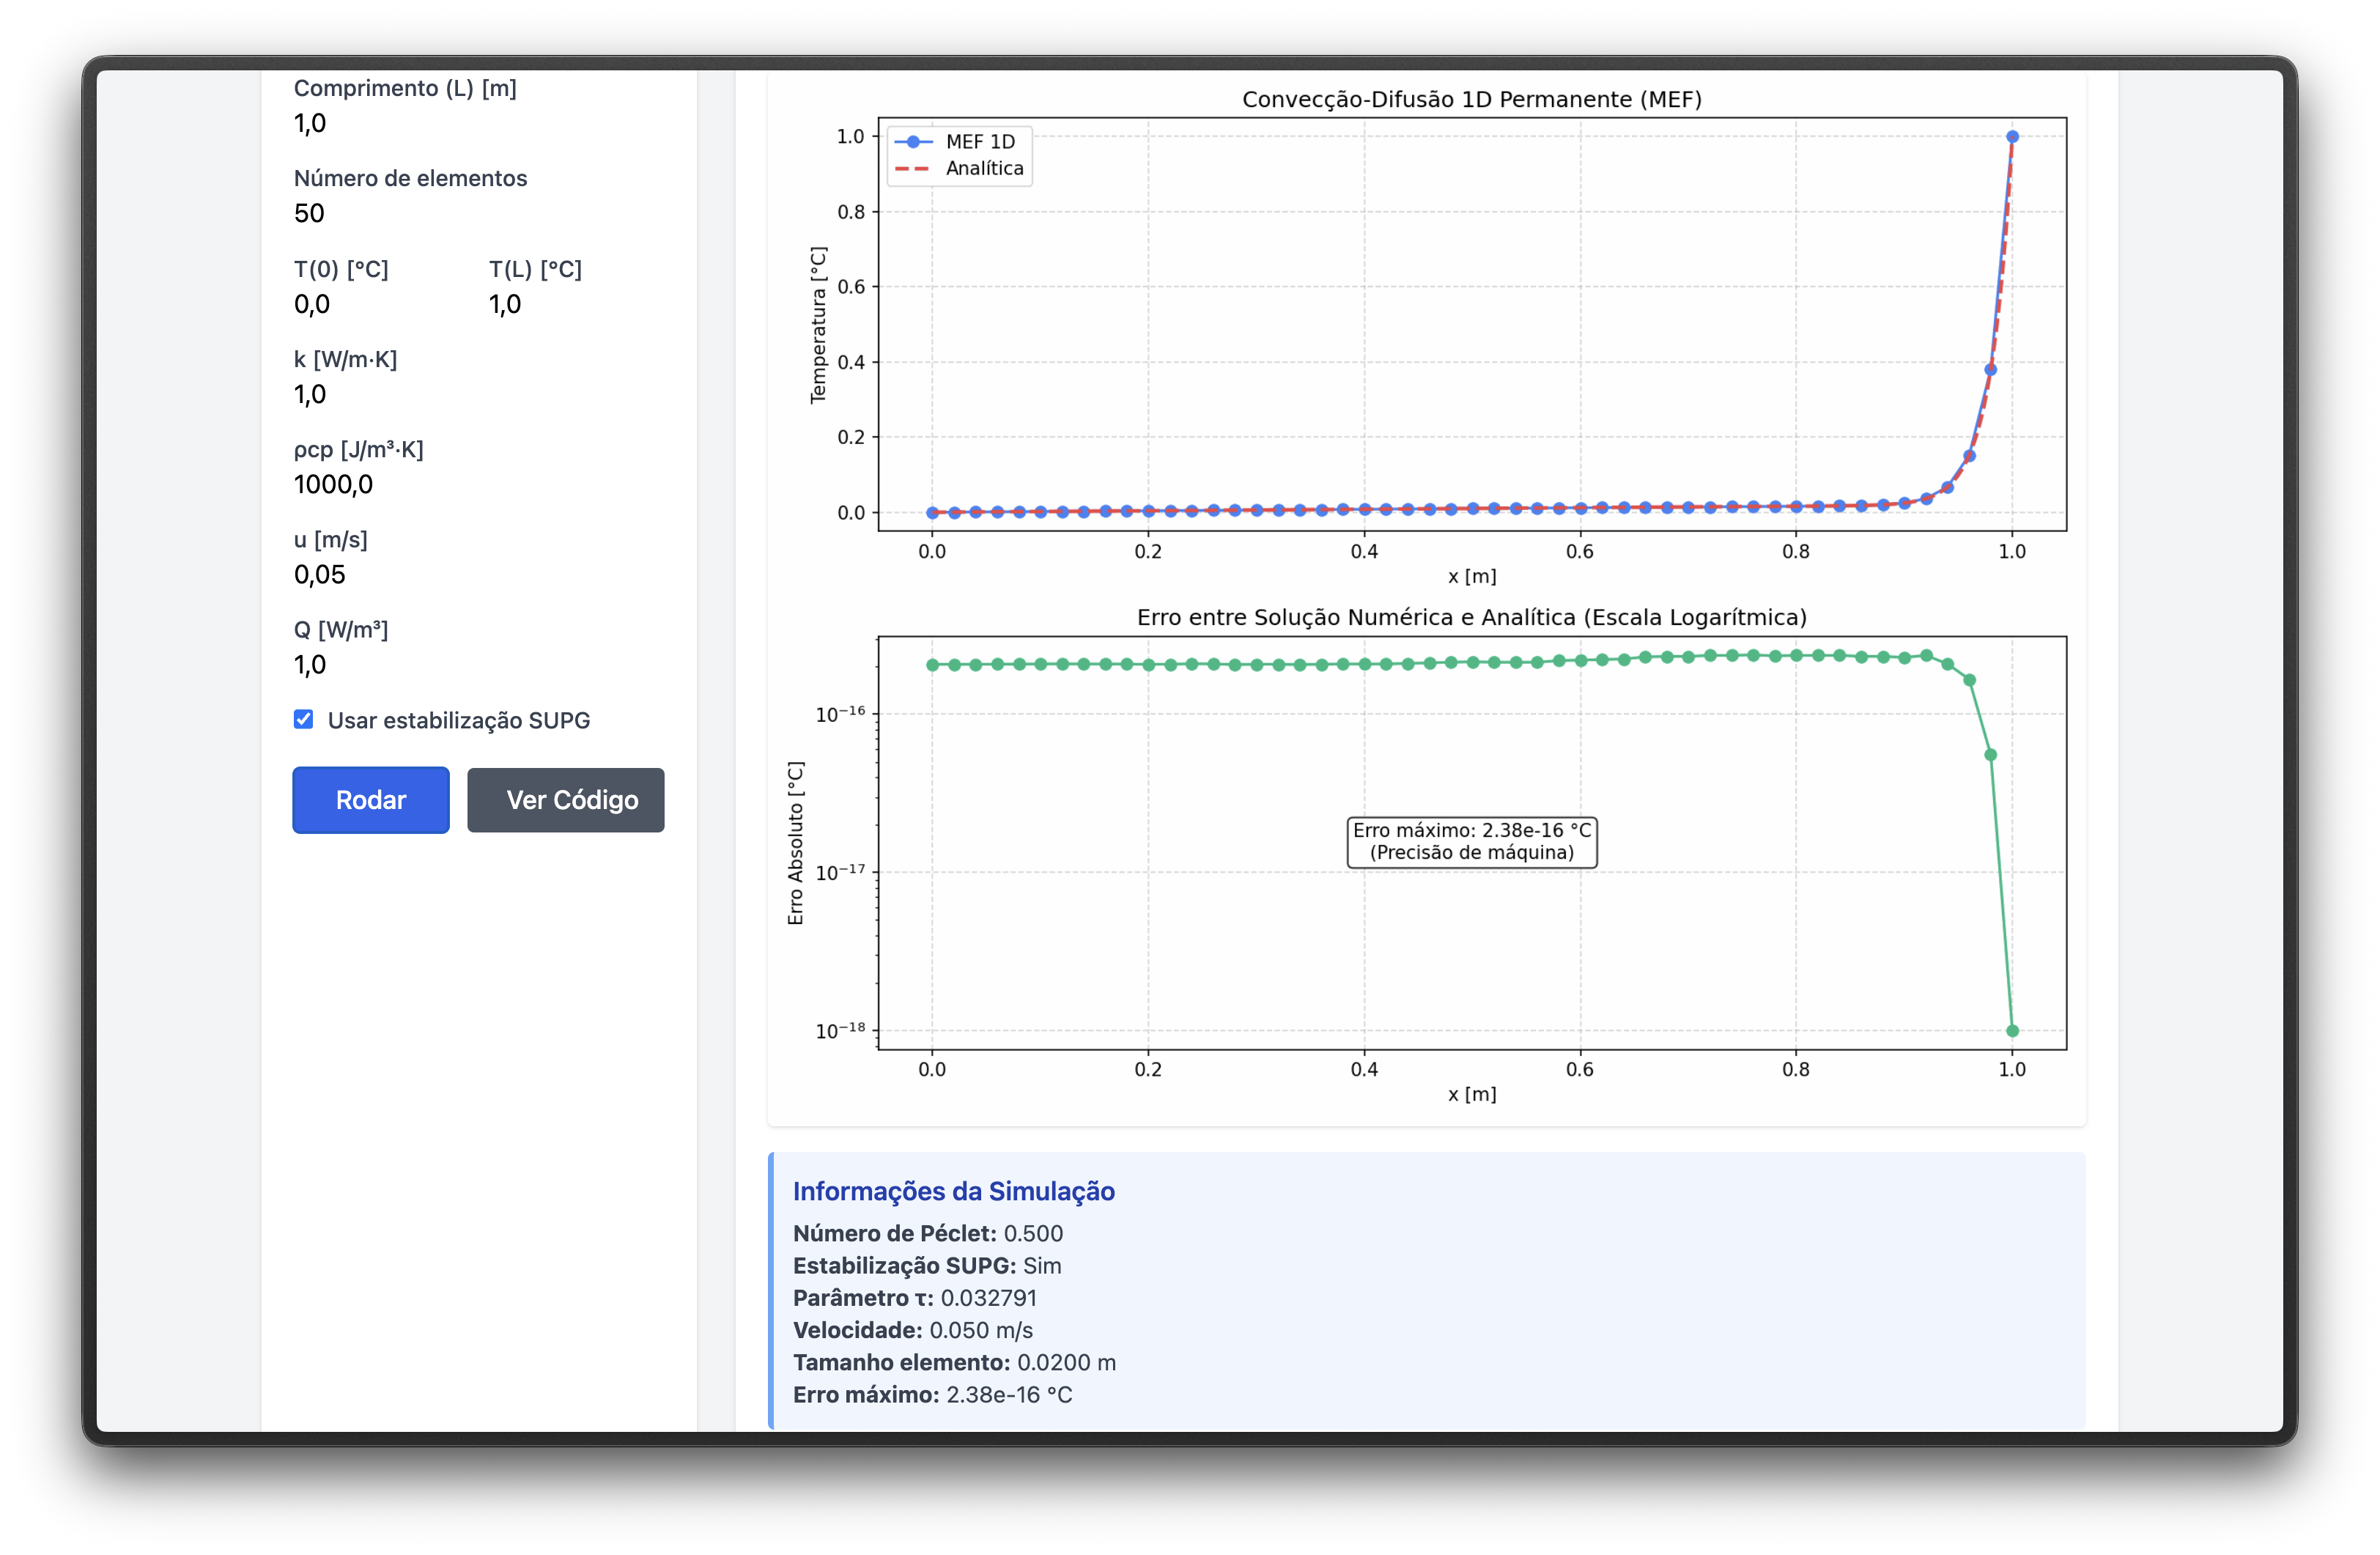
\includegraphics[width=0.85\textwidth]{figuras/prints/fig_convdif1d_com_supg.png}
    \caption{Convecção-difusão 1D com estabilização SUPG ($\text{Pe} \gg 1$): solução MEF comparada à analítica.}
    \label{fig:convdif_supg}
\end{figure}

\subsection{Viga 1D --- Análise de Flexão (Euler-Bernoulli)}
\label{sec:caso_viga}

O módulo de viga 1D implementa elementos finitos de Euler-Bernoulli com dois graus de liberdade por nó: deslocamento vertical $w$ e rotação $\theta$, seguindo o procedimento de Galerkin apresentado na Seção~\ref{sec:galerkin} com funções de interpolação cúbicas de Hermite. A equação governante para a flexão estática é:

\begin{equation}
\frac{d^2}{dx^2}\left( EI \frac{d^2 w}{dx^2} \right) = q(x)
\label{eq:euler_bernoulli}
\end{equation}

A matriz de rigidez elementar $4 \times 4$ é construída com as funções de interpolação cúbicas de Hermite:

\begin{lstlisting}
# Matriz de rigidez do elemento de viga
ke = (EI / h**3) * np.array([
    [12,   6*h,  -12,   6*h  ],
    [6*h,  4*h**2, -6*h, 2*h**2],
    [-12, -6*h,   12,  -6*h  ],
    [6*h,  2*h**2, -6*h, 4*h**2]
])
\end{lstlisting}

O módulo suporta quatro condições de contorno (simplesmente apoiada, balanço, engastada-engastada e engastada-apoiada) e cinco tipos de carregamento (uniforme, linear, triangular, senoidal e pontual), além de propriedades materiais variáveis ao longo do comprimento. A Figura \ref{fig:viga1d_resultado} apresenta a análise completa de uma viga, incluindo deflexão, diagramas de momento fletor e esforço cortante.

\begin{figure}[H]
    \centering
    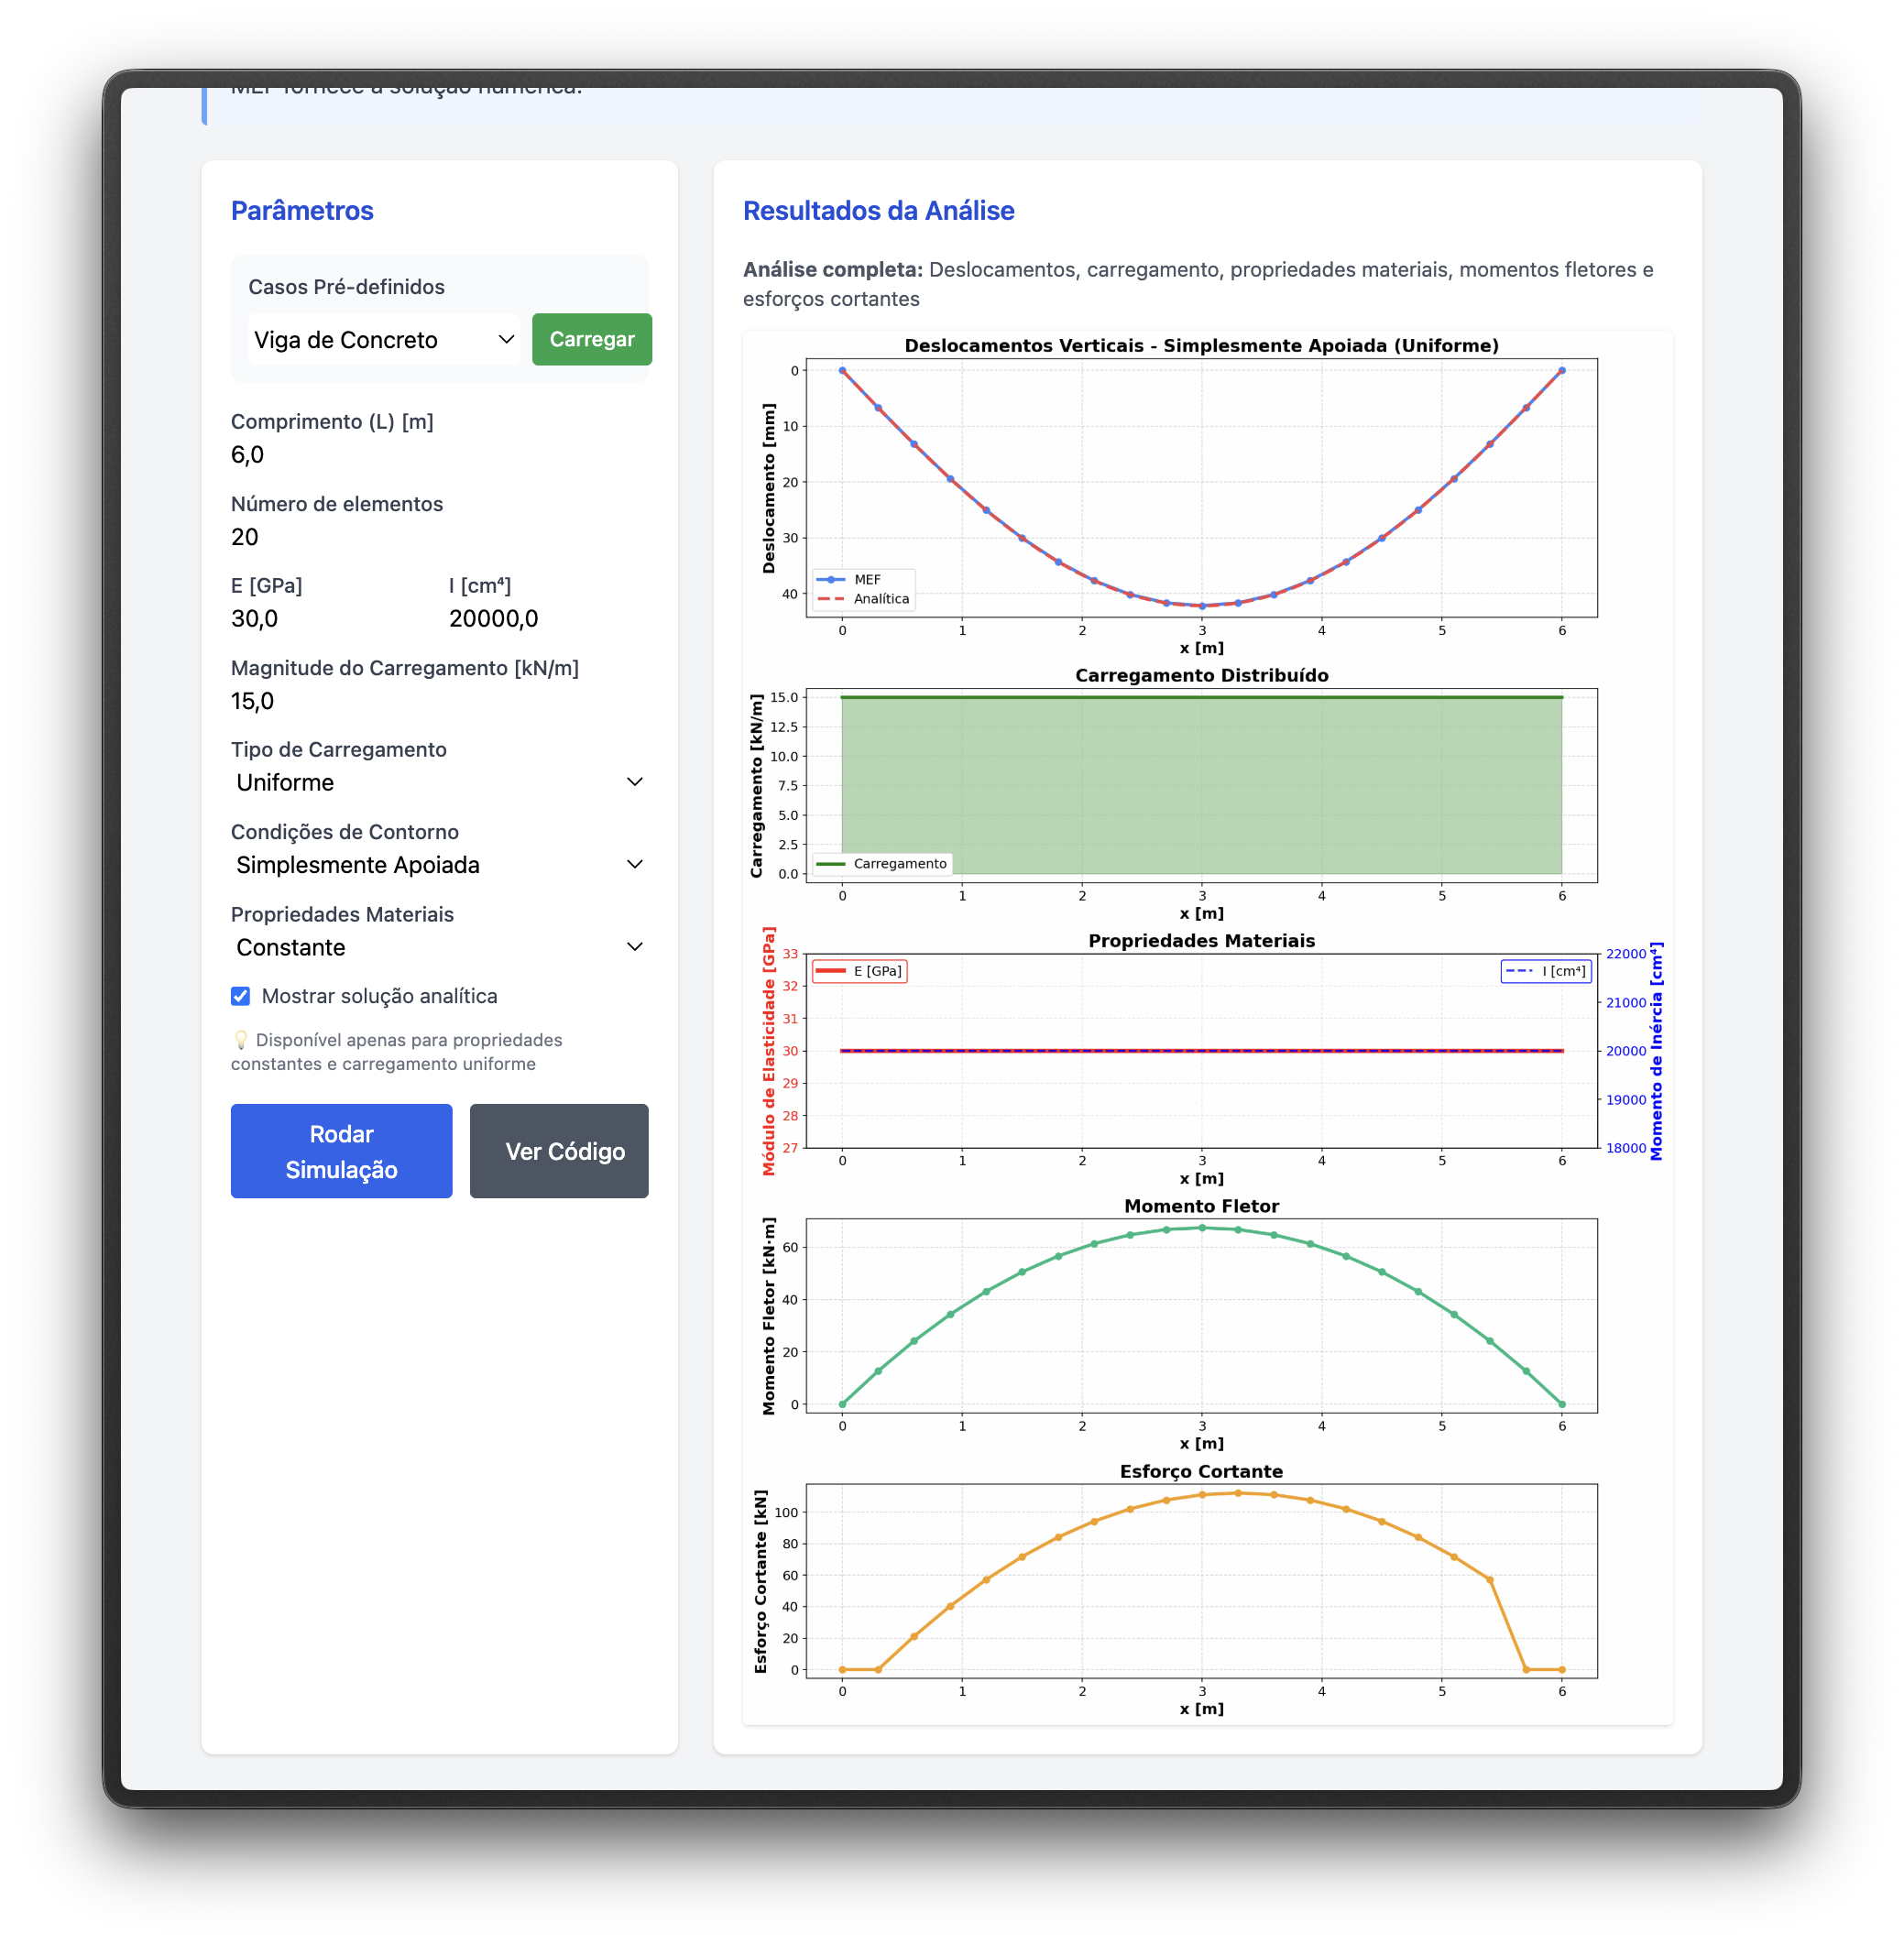
\includegraphics[width=0.85\textwidth]{figuras/prints/fig_viga1d_resultado.png}
    \caption{Análise de flexão de viga 1D (Euler-Bernoulli): deflexão, carregamento, propriedades, momento fletor e esforço cortante.}
    \label{fig:viga1d_resultado}
\end{figure}

\subsection{Vibração 1D --- Problema de Autovalor}
\label{sec:caso_vibracao}

O módulo de vibração resolve o problema de autovalor generalizado $\mathbf{K} \boldsymbol{\phi} = \lambda \, \mathbf{M} \boldsymbol{\phi}$ para uma barra elástica 1D, onde as frequências naturais são $f_n = \sqrt{\lambda_n} / (2\pi)$ e os autovetores $\boldsymbol{\phi}_n$ representam os modos de vibração. As matrizes de rigidez e massa são construídas conforme o procedimento de montagem global descrito na Seção~\ref{sec:montagem_global}, empregando massa concentrada (\textit{lumped}, Eq.~\ref{eq:massa_lumped}):

\begin{lstlisting}
# Matrizes de rigidez e massa (barra 1D)
ke = (E*A / h) * np.array([[1, -1], [-1, 1]])
me = (rho*A*h / 2) * np.array([[1, 0], [0, 1]])
\end{lstlisting}

O problema de autovalor é resolvido pela rotina \texttt{scipy.linalg.eigh}, que explora a simetria das matrizes para eficiência e estabilidade numérica. A solução fornece $n$ frequências naturais e os correspondentes modos de vibração, comparáveis com as expressões analíticas clássicas --- por exemplo, $f_n = n c / (2L)$ para barras engastadas em ambas as extremidades, onde $c = \sqrt{E/\rho}$ é a velocidade de propagação de ondas. A Figura \ref{fig:vibracao1d_modos} ilustra os cinco primeiros modos.

\begin{figure}[H]
    \centering
    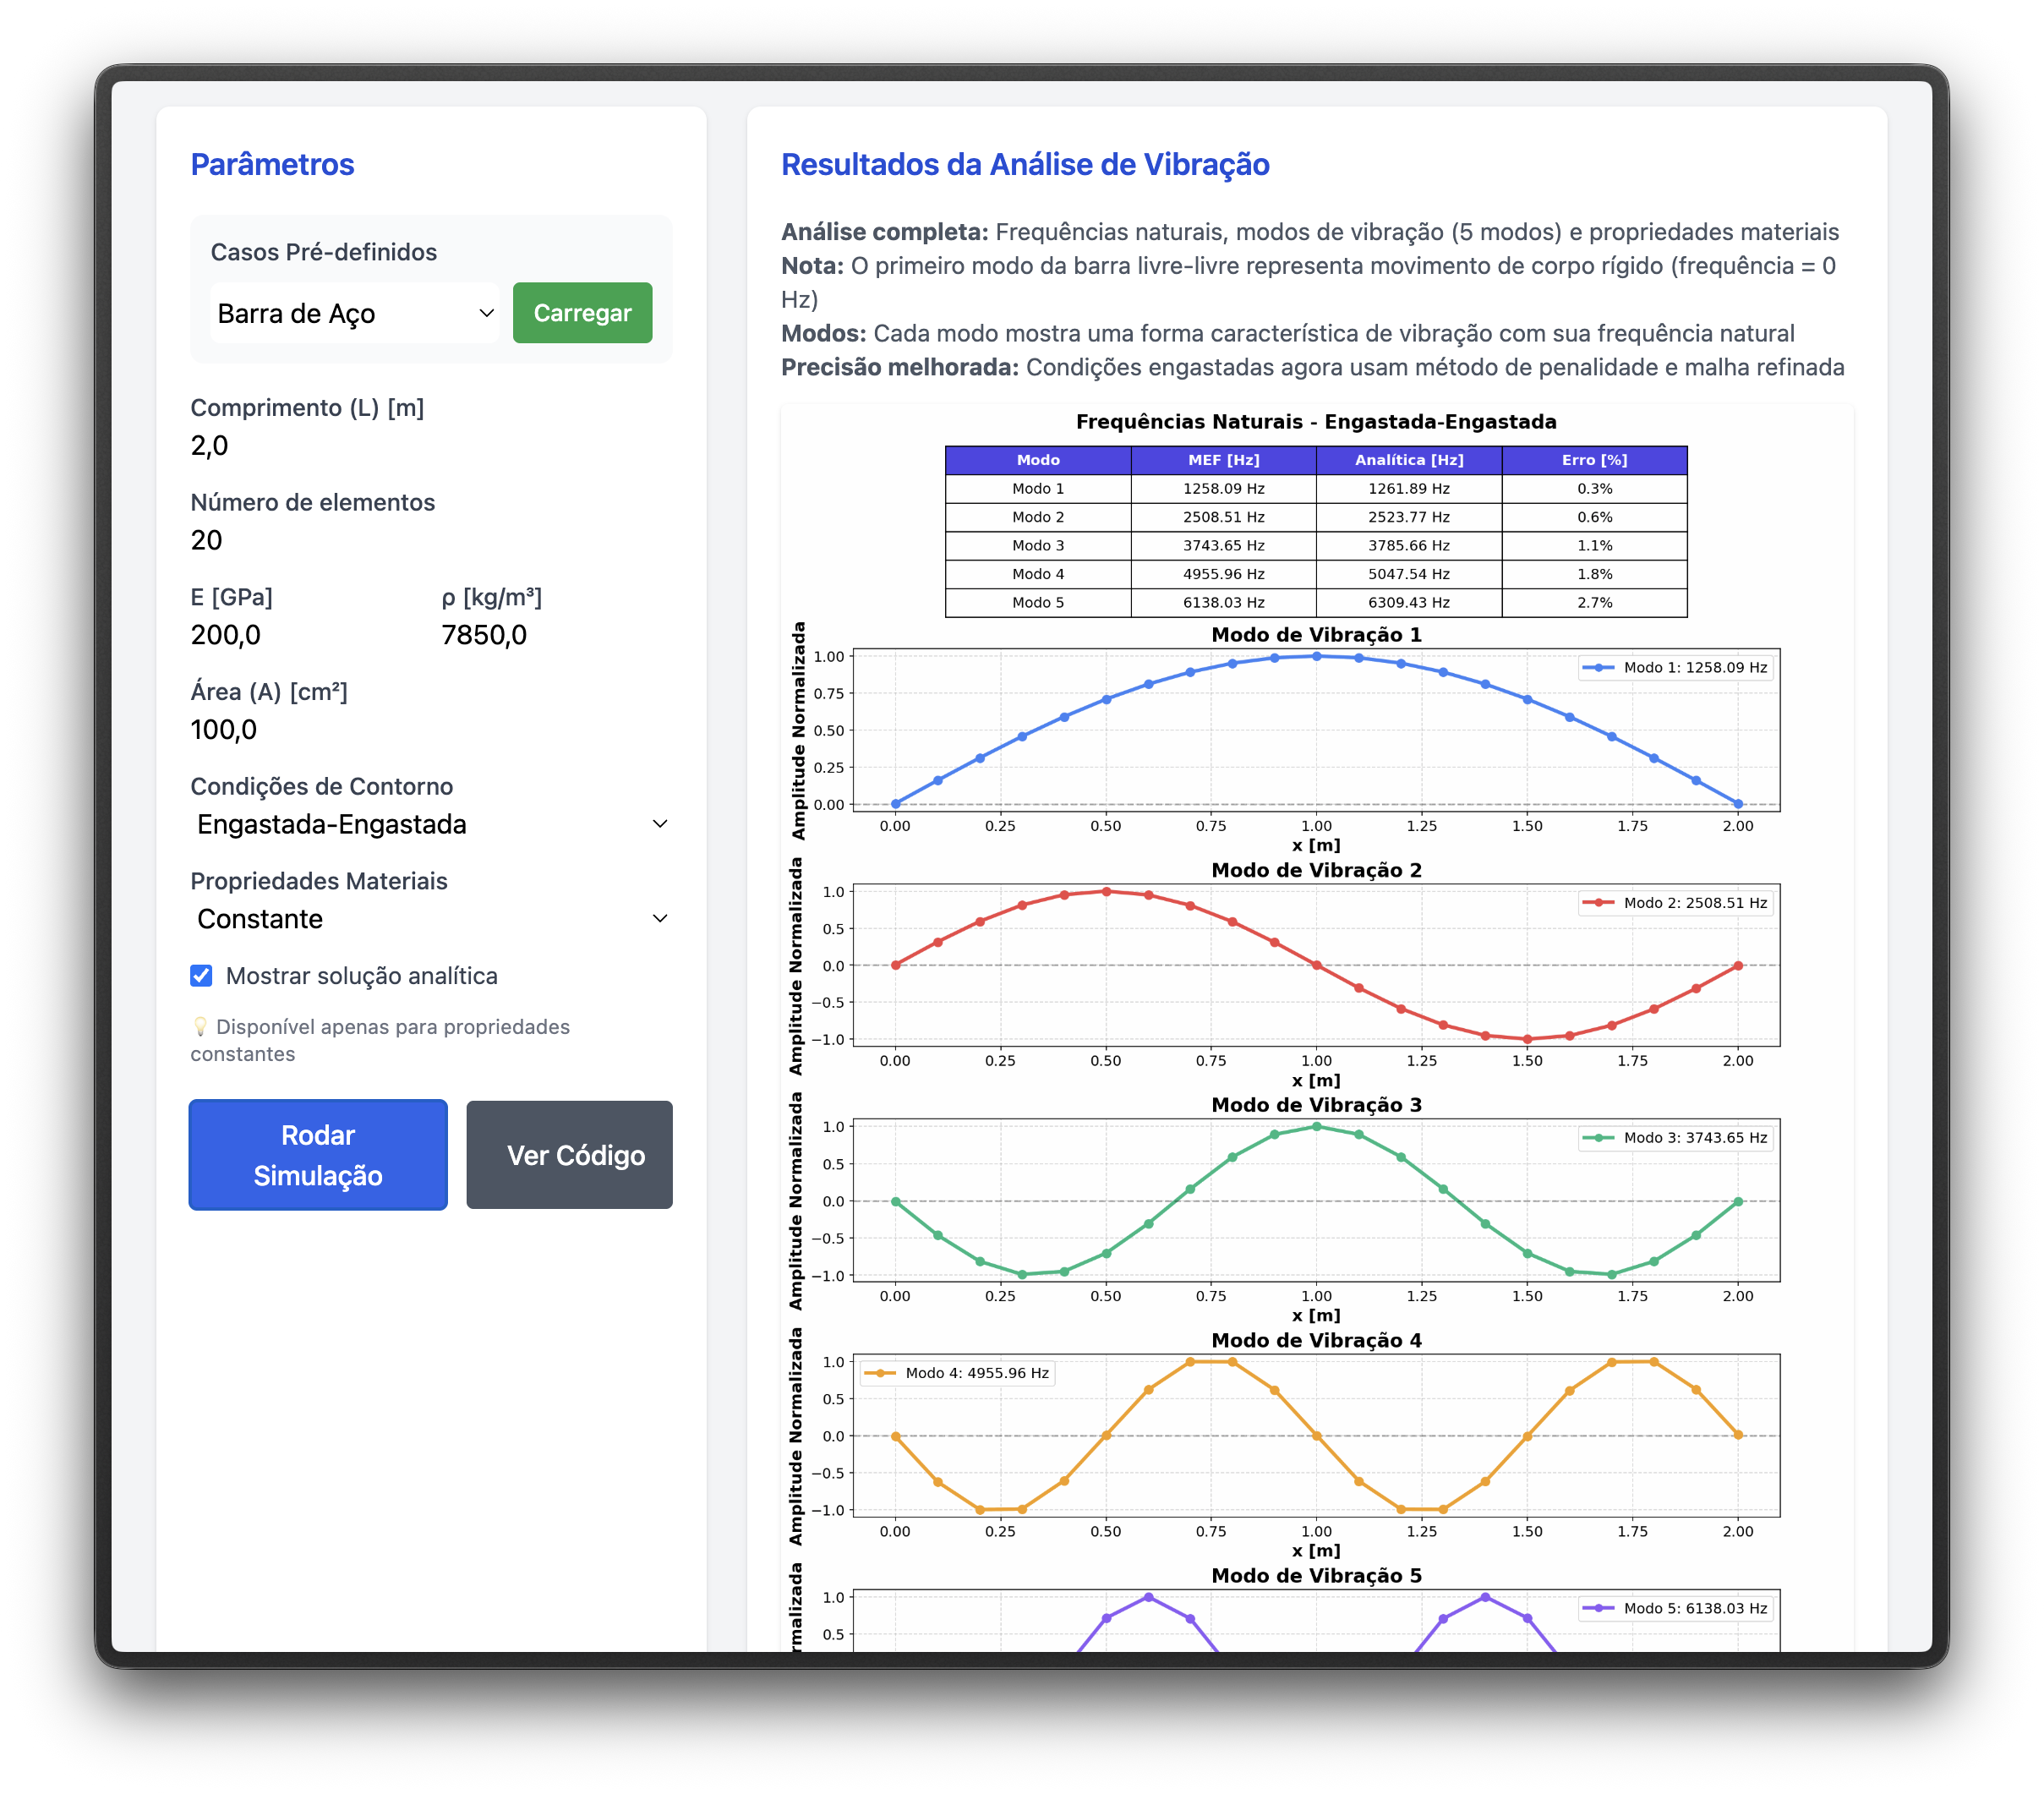
\includegraphics[width=0.85\textwidth]{figuras/prints/fig_vibracao1d_modos.png}
    \caption{Frequências naturais e cinco primeiros modos de vibração de uma barra 1D.}
    \label{fig:vibracao1d_modos}
\end{figure}

\subsection{Transferência de Calor 2D}
\label{sec:caso_transcalor}

O módulo de transferência de calor bidimensional resolve a equação de condução transiente em uma placa quadrada discretizada com elementos triangulares P1 (Seção~\ref{sec:elementos_p1}). As matrizes elementares de rigidez e massa são construídas pela função compartilhada \texttt{element\_matrices}, que implementa diretamente as expressões derivadas na Seção~\ref{sec:matrizes_elementares} (Eqs.~\ref{eq:rigidez_elementar} e~\ref{eq:massa_elementar}):

\begin{lstlisting}
def element_matrices(coords, k, rho, cv):
    x0, x1, x2 = coords
    area = 0.5 * abs((x1[0]-x0[0])*(x2[1]-x0[1])
                    -(x2[0]-x0[0])*(x1[1]-x0[1]))
    b = np.array([x1[1]-x2[1], x2[1]-x0[1], x0[1]-x1[1]])
    c = np.array([x2[0]-x1[0], x0[0]-x2[0], x1[0]-x0[0]])
    ke = (k/(4*area)) * (np.outer(b,b) + np.outer(c,c))
    me = (rho*cv*area/12) * (np.ones((3,3)) + np.eye(3))
    return ke, me
\end{lstlisting}

A integração temporal emprega o método de Crank-Nicolson ($\theta = 1/2$), conforme a formulação do método $\theta$ generalizado apresentada na Seção~\ref{sec:integracao_temporal} (Eq.~\ref{eq:theta_method}), formulado com matrizes esparsas (\texttt{scipy.sparse}) para viabilizar a execução no navegador com malhas de até $40 \times 40$ nós. A cada passo de tempo, um frame do campo de temperatura é gerado e acumulado para compor uma animação GIF. A Figura \ref{fig:transcalor2d_campo} ilustra um instante da evolução temporal.

\begin{figure}[H]
    \centering
    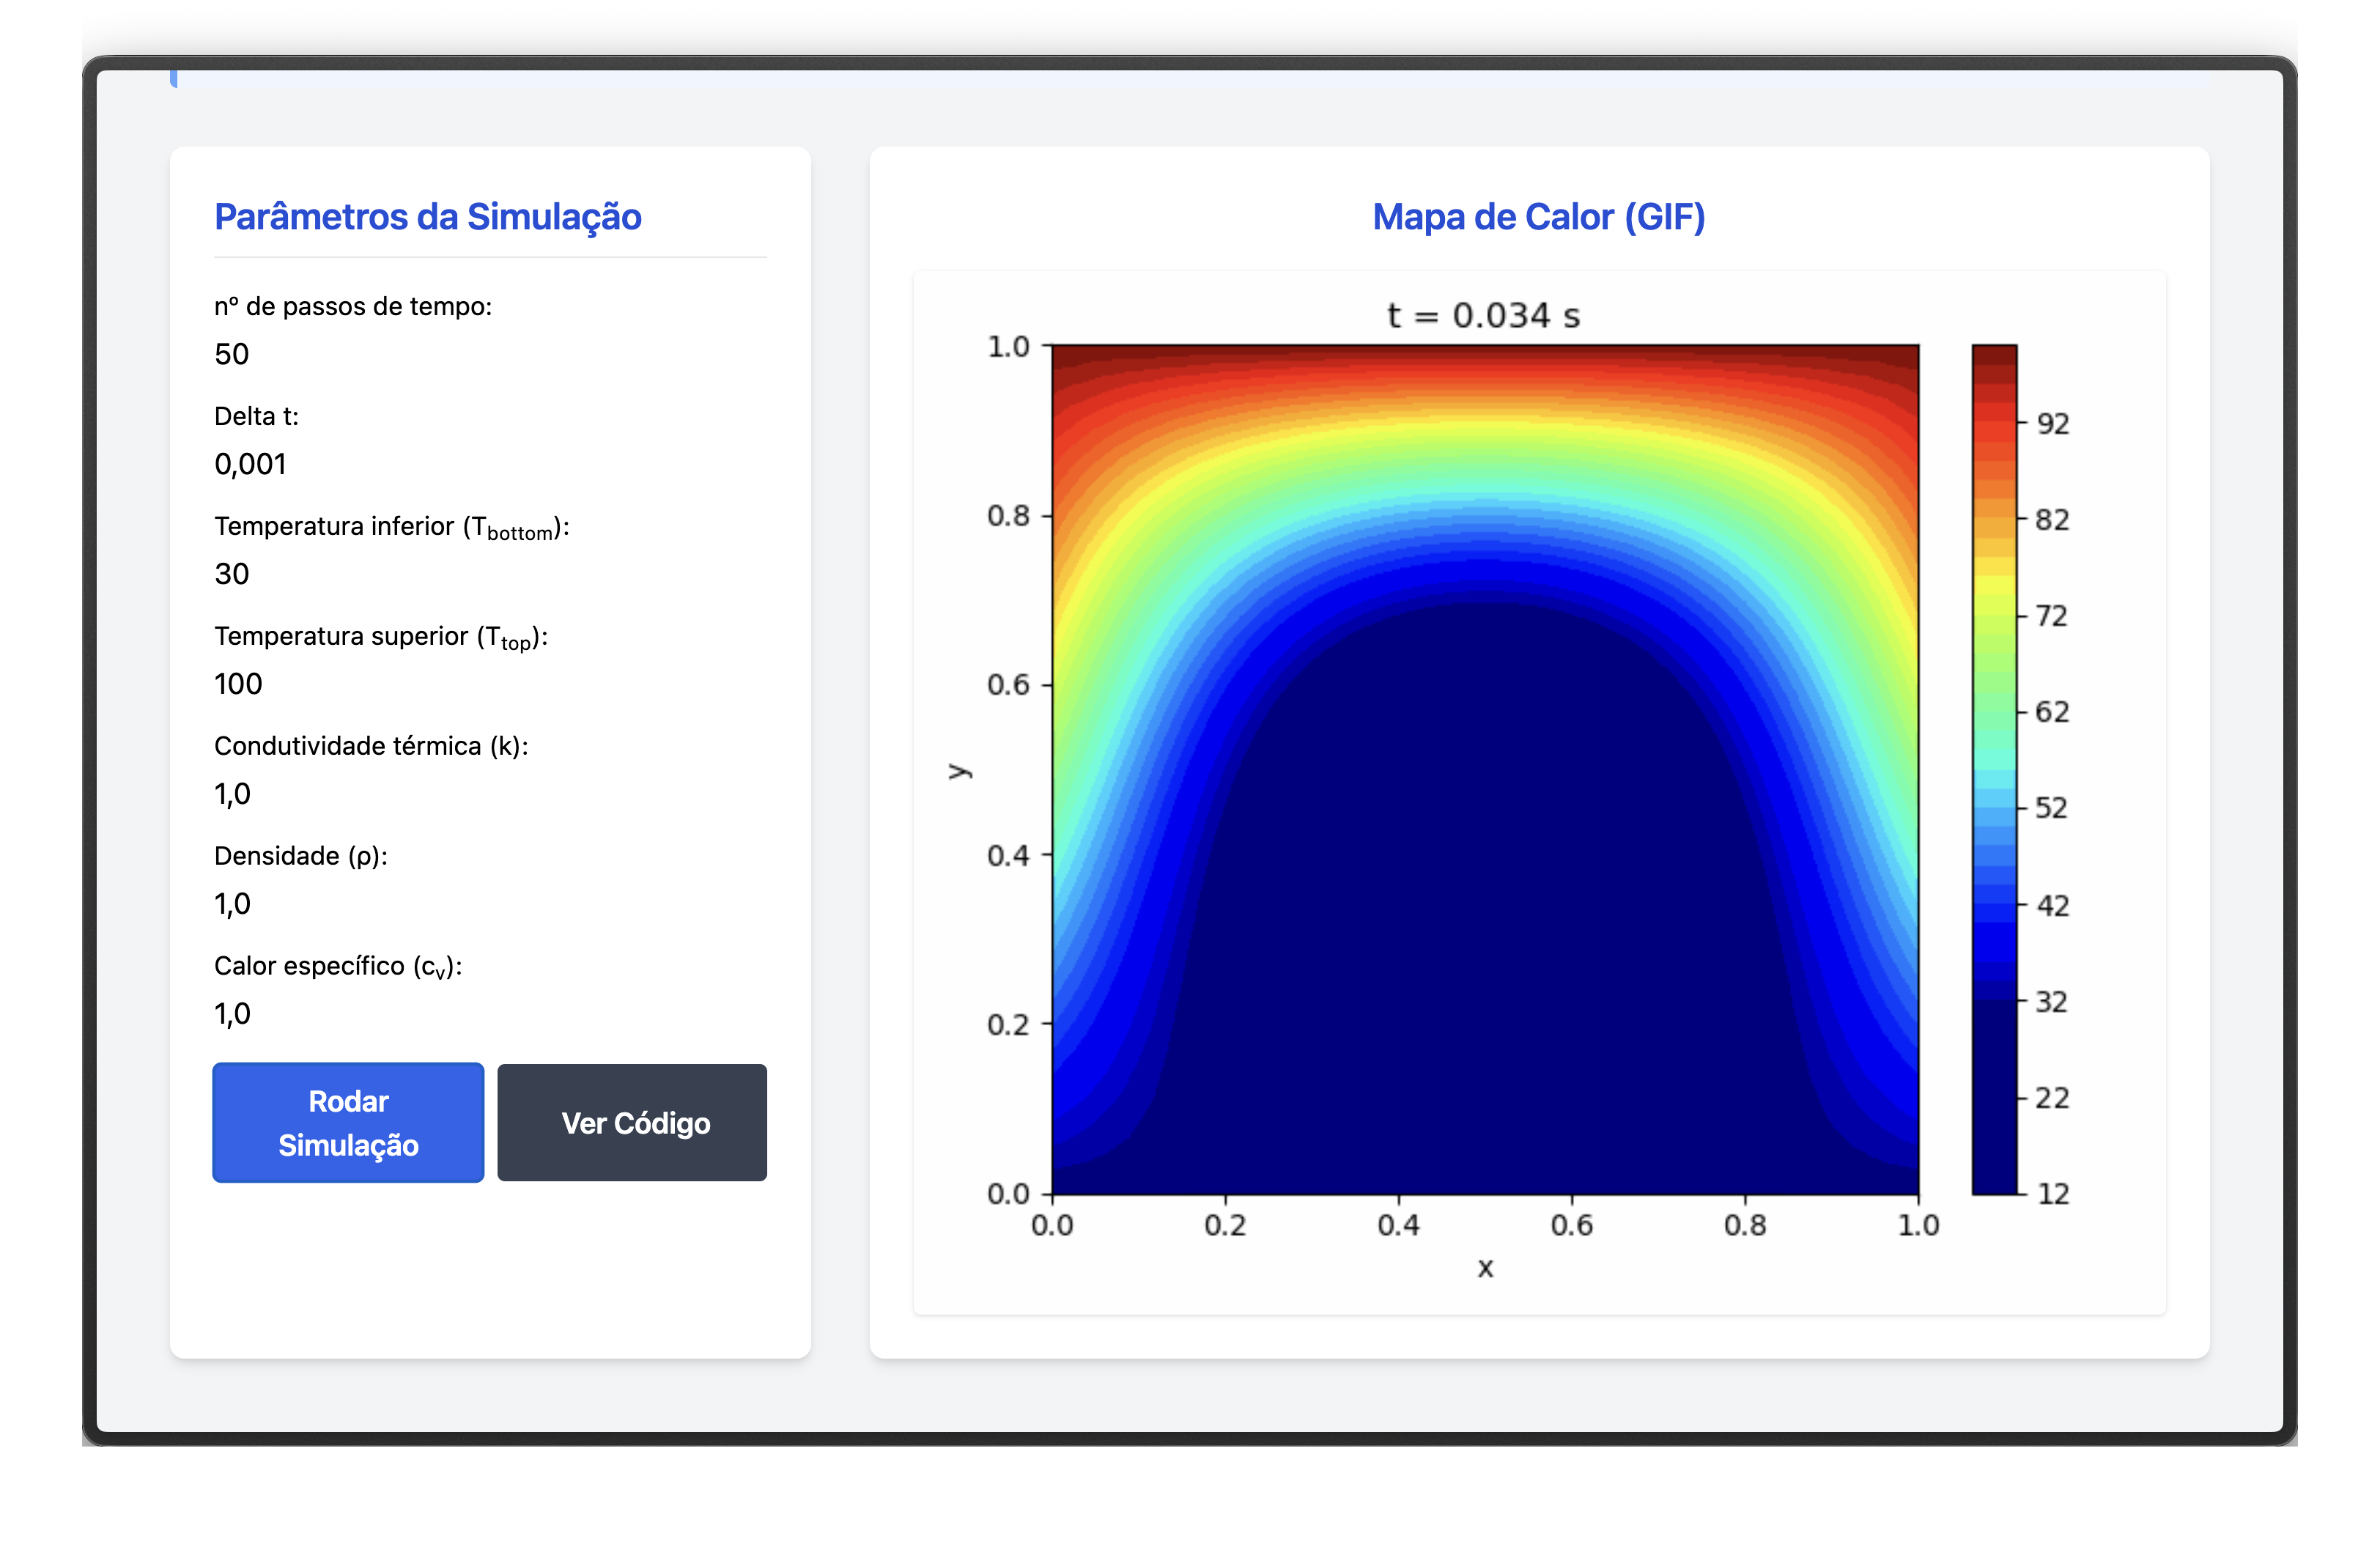
\includegraphics[width=0.75\textwidth]{figuras/prints/fig_transcalor2d_campo.png}
    \caption{Campo de temperatura em placa 2D durante a evolução transiente (método de Crank-Nicolson).}
    \label{fig:transcalor2d_campo}
\end{figure}

\subsection{Escoamento Potencial 2D}
\label{sec:caso_potencial}

O módulo de escoamento potencial resolve a equação de Laplace $\nabla^2 \psi = 0$ em domínios 2D com obstáculos, caso particular da equação de Poisson para a função corrente (Eq.~\ref{eq:poisson_psi}) com vorticidade nula. A malha triangular é gerada pelo módulo \texttt{common.py}, que também assembla as matrizes globais de rigidez e massa conforme o procedimento descrito na Seção~\ref{sec:montagem_global}.

O módulo \texttt{geometry.py} fornece diferentes geometrias de obstáculo (cilindro, retângulo, degrau), sendo os nós do contorno do obstáculo inseridos na malha com a condição $\psi = \text{constante}$. As velocidades são recuperadas por:

\begin{equation}
u = \frac{\partial \psi}{\partial y} \approx \frac{1}{2A^e} \sum_j \psi_j c_j, \qquad v = -\frac{\partial \psi}{\partial x} \approx -\frac{1}{2A^e} \sum_j \psi_j b_j
\label{eq:vel_recuperacao}
\end{equation}

A Figura \ref{fig:potencial2d_linhas} apresenta as linhas de corrente para escoamento ao redor de um obstáculo.

\begin{figure}[H]
    \centering
    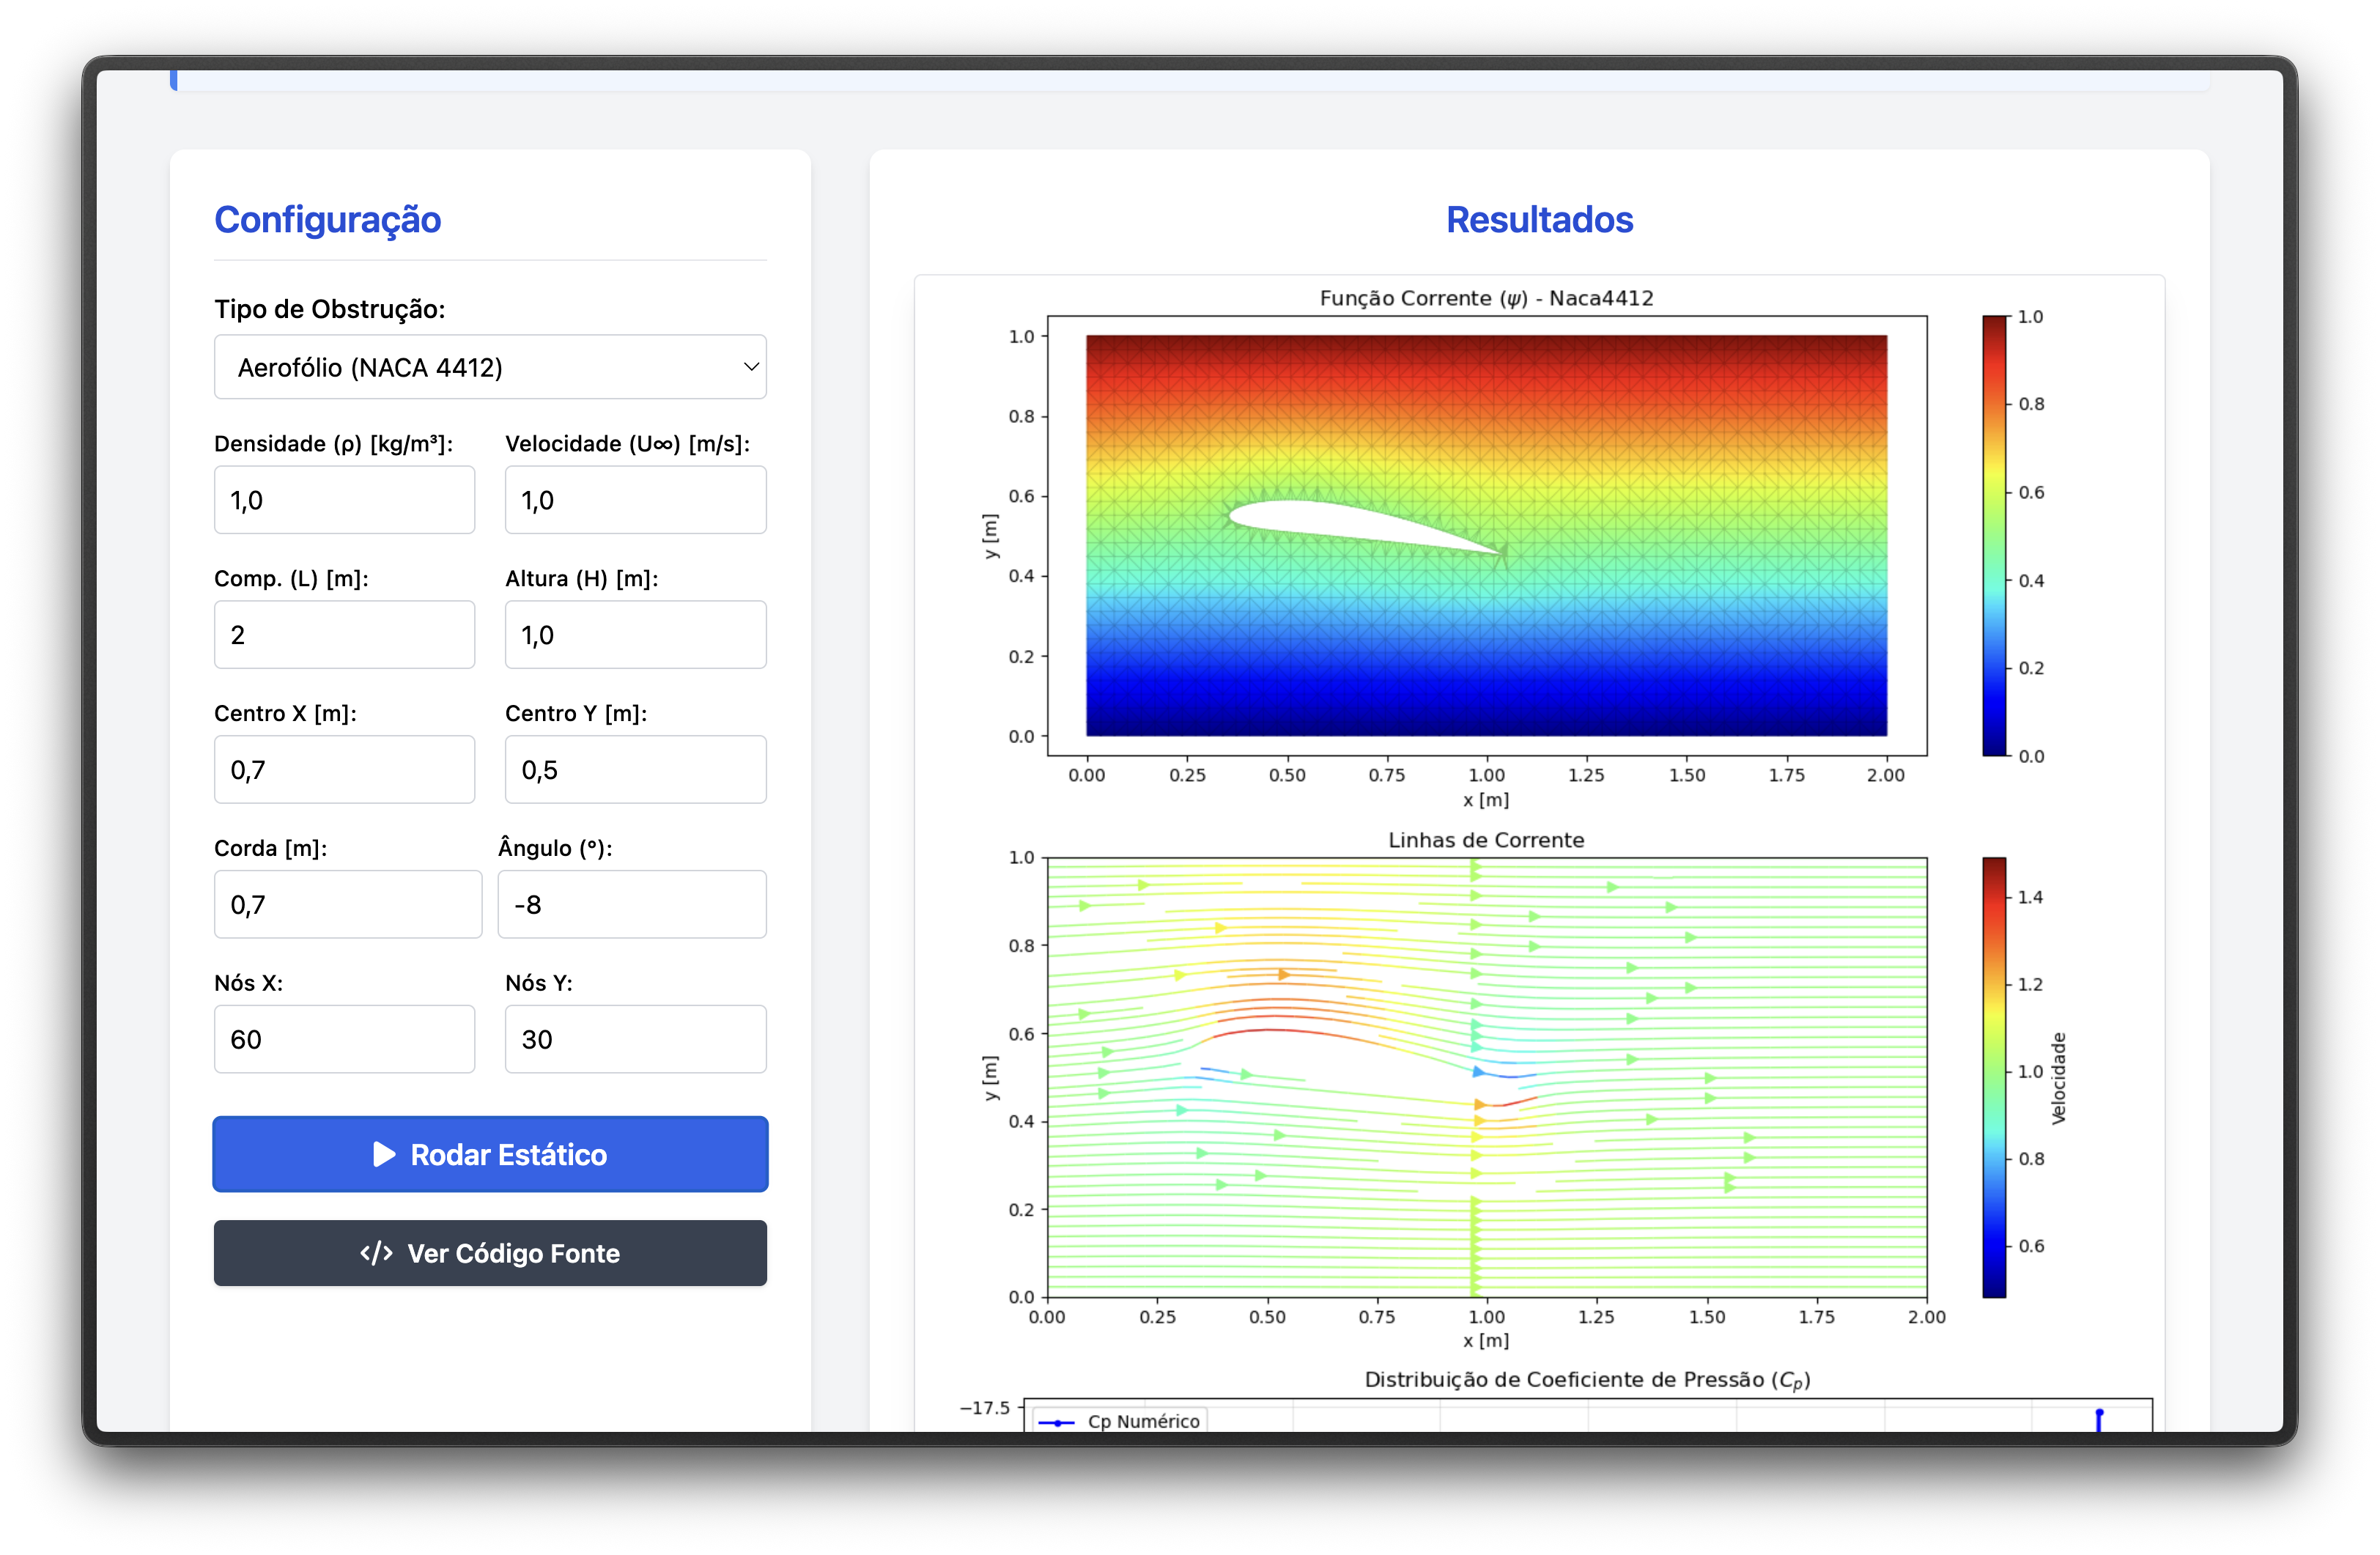
\includegraphics[width=0.85\textwidth]{figuras/prints/fig_potencial2d_linhas.png}
    \caption{Escoamento potencial 2D: linhas de corrente ao redor de um obstáculo.}
    \label{fig:potencial2d_linhas}
\end{figure}

\subsection{Navier-Stokes 2D (Vorticidade-Corrente)}
\label{sec:caso_ns}

O módulo mais complexo da plataforma implementa o solver de Navier-Stokes 2D na formulação Vorticidade-Corrente ($\omega$-$\psi$), conforme descrito na Seção~\ref{sec:vorticidade_corrente}. A discretização temporal segue o esquema semi-implícito derivado na Seção~\ref{sec:semi_implicito} (Eq.~\ref{eq:sistema_temporal_ns}), enquanto as condições de contorno de vorticidade nas paredes são impostas conforme a Eq.~\ref{eq:thom}. O algoritmo segue o procedimento iterativo:

\begin{enumerate}
    \item Resolver a equação de Poisson $\mathbf{K} \boldsymbol{\psi} = \mathbf{M} \boldsymbol{\omega}$ para $\psi$;
    \item Atualizar a vorticidade nas paredes sólidas conforme a Eq.~\ref{eq:thom};
    \item Calcular $(u, v)$ a partir de $\psi$ (Eq.~\ref{eq:vel_recuperacao});
    \item Assemblar a matriz de convecção $\mathbf{C}^n$ com o campo de velocidades atual;
    \item Resolver o transporte da vorticidade pelo esquema semi-implícito (Eq.~\ref{eq:sistema_temporal_ns}).
\end{enumerate}

O solver suporta dois cenários: escoamento em canal com obstáculos (cilindro, retângulo, degrau) e cavidade com tampa móvel (\textit{lid-driven cavity}). No caso da cavidade, todas as paredes possuem $\psi = 0$ e a parede superior impõe velocidade tangencial $u_{\text{lid}} = 1$, acrescentando o termo $-2u_{\text{tan}}/h$ à condição de contorno da vorticidade. A Figura \ref{fig:ns2d_cavity} mostra os campos de $\psi$, $\omega$ e as linhas de corrente para a cavidade a $\text{Re} = 100$.

\begin{figure}[H]
    \centering
    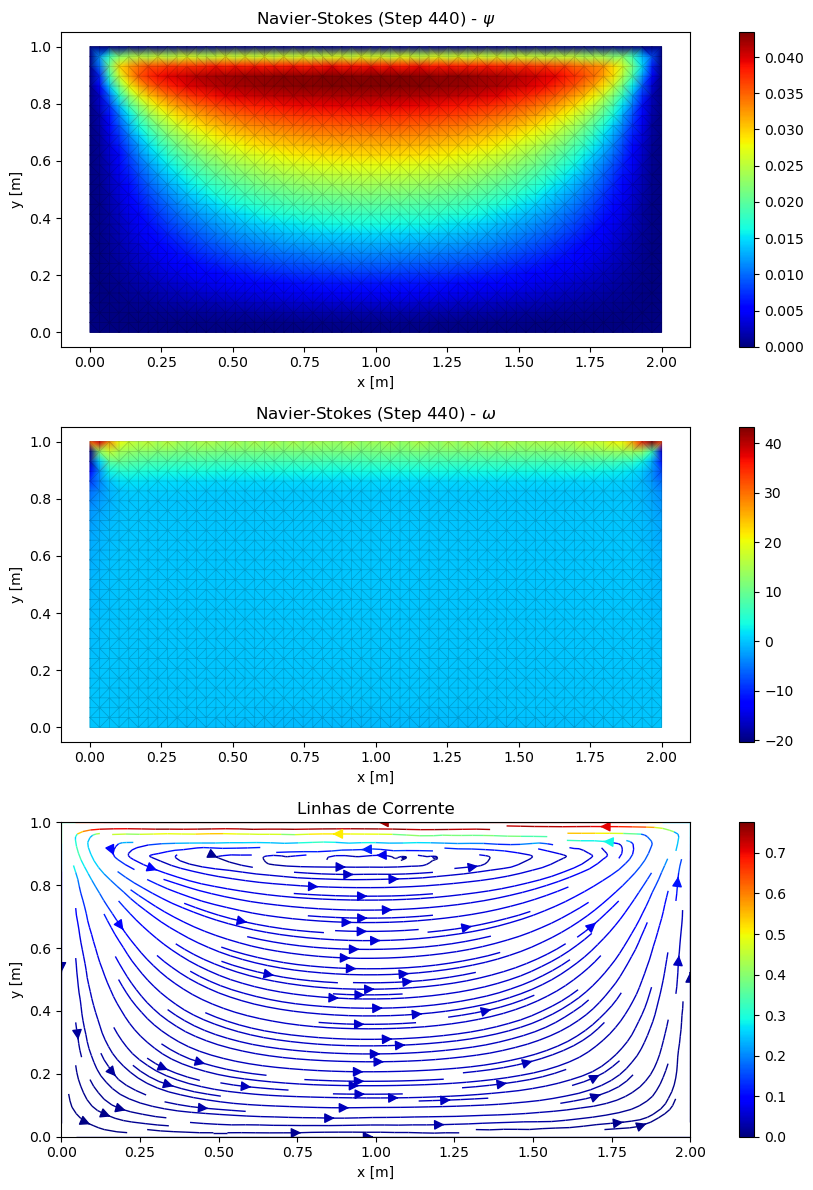
\includegraphics[width=0.85\textwidth]{figuras/prints/fig_ns2d_cavity_re100.png}
    \caption{Navier-Stokes 2D --- cavidade com tampa móvel ($\text{Re} = 100$): campos de $\psi$, $\omega$ e linhas de corrente.}
    \label{fig:ns2d_cavity}
\end{figure}

\begin{figure}[H]
    \centering
    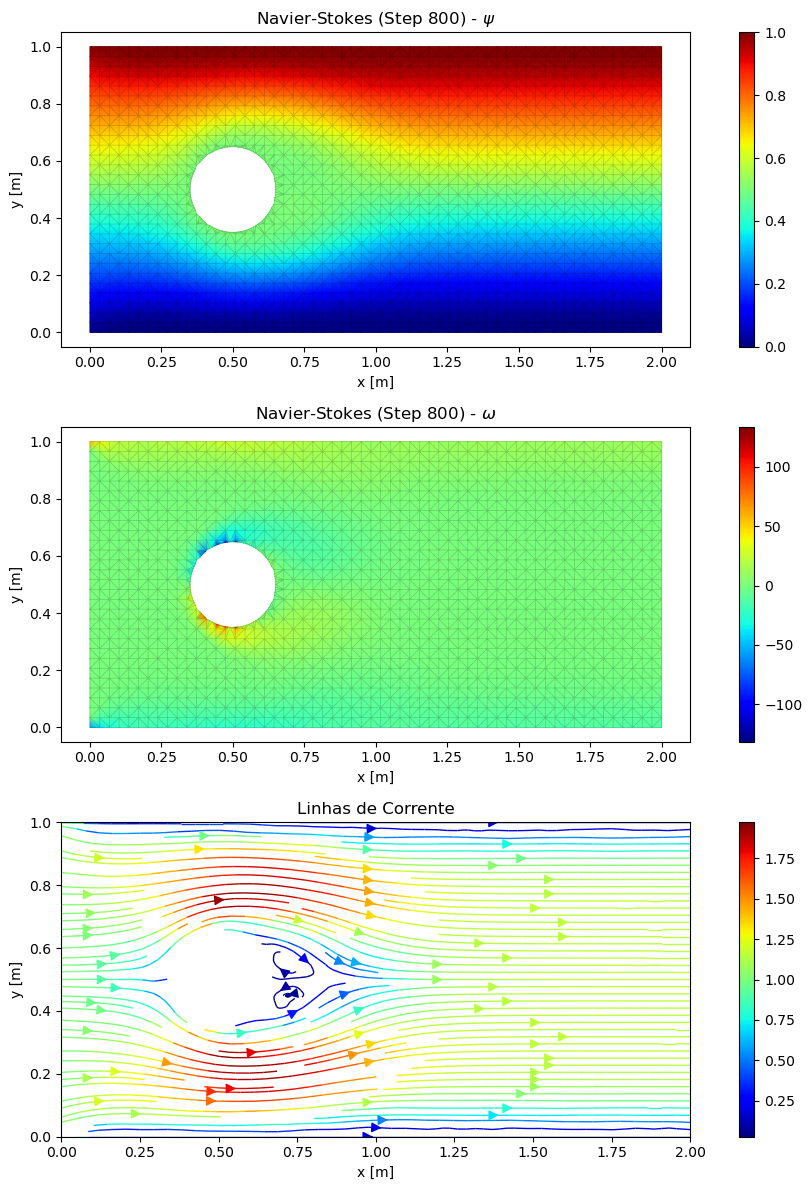
\includegraphics[width=0.85\textwidth]{figuras/prints/fig_ns2d_cylinder.png}
    \caption{Navier-Stokes 2D --- linhas de corrente para escoamento ao redor de um cilindro.}
    \label{fig:ns2d_cylinder}
\end{figure}

\section{Síntese do Capítulo}
\label{sec:sintese_arquitetura}

\paragraph{}Do ponto de vista da integração teórico-computacional, todos os módulos descritos neste capítulo compartilham o mesmo núcleo numérico: construção de matrizes elementares, montagem global por conectividade nodal, solução de sistemas lineares e, nos casos transientes, avanço temporal via método $\theta$ ou esquema semi-implícito. Dessa forma, a plataforma \textit{MinervaMesh} operacionaliza integralmente o arcabouço teórico estabelecido no Capítulo~\ref{cap3}, mantendo correspondência direta entre as equações governantes contínuas, os sistemas discretizados obtidos pela formulação de Galerkin e os \textit{solvers} efetivamente implementados. As listagens completas dos códigos, apresentadas nos Apêndices~\ref{ApendiceA} e~\ref{ApendiceB}, documentam essa correspondência em nível de implementação linha a linha.

\paragraph{}Este capítulo apresentou a arquitetura e a implementação do \textit{MinervaMesh}. A escolha do PyScript e da computação \textit{client-side} viabiliza uma plataforma de simulação numérica com custo de infraestrutura zero, portabilidade total e código aberto para inspeção acadêmica. A organização modular do repositório --- com cada simulação autocontida em três arquivos (HTML, Python, TOML) --- permite a extensão da plataforma com novos casos sem impacto nos módulos existentes. Os oito módulos MEF descritos cobrem três domínios da Engenharia Mecânica (térmico, estrutural e fluidodinâmico), demonstrando a versatilidade da formulação de elementos finitos apresentada no Capítulo 3. O Capítulo 5 apresentará a validação quantitativa desses módulos através da comparação com soluções analíticas e benchmarks da literatura.
